%% bare_jrnl.tex
%% V1.4b
%% 2015/08/26
%% by Michael Shell
%% see http://www.michaelshell.org/
%% for current contact information.
%%
%% This is a skeleton file demonstrating the use of IEEEtran.cls
%% (requires IEEEtran.cls version 1.8b or later) with an IEEE
%% journal paper.
%%
%% Support sites:
%% http://www.michaelshell.org/tex/ieeetran/
%% http://www.ctan.org/pkg/ieeetran
%% and
%% http://www.ieee.org/

%%*************************************************************************
%% Legal Notice:
%% This code is offered as-is without any warranty either expressed or
%% implied; without even the implied warranty of MERCHANTABILITY or
%% FITNESS FOR A PARTICULAR PURPOSE! 
%% User assumes all risk.
%% In no event shall the IEEE or any contributor to this code be liable for
%% any damages or losses, including, but not limited to, incidental,
%% consequential, or any other damages, resulting from the use or misuse
%% of any information contained here.
%%
%% All comments are the opinions of their respective authors and are not
%% necessarily endorsed by the IEEE.
%%
%% This work is distributed under the LaTeX Project Public License (LPPL)
%% ( http://www.latex-project.org/ ) version 1.3, and may be freely used,
%% distributed and modified. A copy of the LPPL, version 1.3, is included
%% in the base LaTeX documentation of all distributions of LaTeX released
%% 2003/12/01 or later.
%% Retain all contribution notices and credits.
%% ** Modified files should be clearly indicated as such, including  **
%% ** renaming them and changing author support contact information. **
%%*************************************************************************


% *** Authors should verify (and, if needed, correct) their LaTeX system  ***
% *** with the testflow diagnostic prior to trusting their LaTeX platform ***
% *** with production work. The IEEE's font choices and paper sizes can   ***
% *** trigger bugs that do not appear when using other class files.       ***                          ***
% The testflow support page is at:
% http://www.michaelshell.org/tex/testflow/

\documentclass[journal]{IEEEtran}
%
% If IEEEtran.cls has not been installed into the LaTeX system files,
% manually specify the path to it like:
% \documentclass[journal]{../sty/IEEEtran}





% Some very useful LaTeX packages include:
% (uncomment the ones you want to load)


% *** MISC UTILITY PACKAGES ***
%
\usepackage{ifpdf}
% Heiko Oberdiek's ifpdf.sty is very useful if you need conditional
% compilation based on whether the output is pdf or dvi.
% usage:
% \ifpdf
%   % pdf code
% \else
%   % dvi code
% \fi
% The latest version of ifpdf.sty can be obtained from:
% http://www.ctan.org/pkg/ifpdf
% Also, note that IEEEtran.cls V1.7 and later provides a builtin
% \ifCLASSINFOpdf conditional that works the same way.
% When switching from latex to pdflatex and vice-versa, the compiler may
% have to be run twice to clear warning/error messages.






% *** CITATION PACKAGES ***
%
\usepackage{cite}
% cite.sty was written by Donald Arseneau
% V1.6 and later of IEEEtran pre-defines the format of the cite.sty package
% \cite{} output to follow that of the IEEE. Loading the cite package will
% result in citation numbers being automatically sorted and properly
% "compressed/ranged". e.g., [1], [9], [2], [7], [5], [6] without using
% cite.sty will become [1], [2], [5]--[7], [9] using cite.sty. cite.sty's
% \cite will automatically add leading space, if needed. Use cite.sty's
% noadjust option (cite.sty V3.8 and later) if you want to turn this off
% such as if a citation ever needs to be enclosed in parenthesis.
% cite.sty is already installed on most LaTeX systems. Be sure and use
% version 5.0 (2009-03-20) and later if using hyperref.sty.
% The latest version can be obtained at:
% http://www.ctan.org/pkg/cite
% The documentation is contained in the cite.sty file itself.






% *** GRAPHICS RELATED PACKAGES ***
%
\ifCLASSINFOpdf
  \usepackage[pdftex]{graphicx}
  % declare the path(s) where your graphic files are
  % \graphicspath{{../pdf/}{../jpeg/}}
  % and their extensions so you won't have to specify these with
  % every instance of \includegraphics
  % \DeclareGraphicsExtensions{.pdf,.jpeg,.png}
\else
  % or other class option (dvipsone, dvipdf, if not using dvips). graphicx
  % will default to the driver specified in the system graphics.cfg if no
  % driver is specified.
  % \usepackage[dvips]{graphicx}
  % declare the path(s) where your graphic files are
  % \graphicspath{{../eps/}}
  % and their extensions so you won't have to specify these with
  % every instance of \includegraphics
  % \DeclareGraphicsExtensions{.eps}
\fi
% graphicx was written by David Carlisle and Sebastian Rahtz. It is
% required if you want graphics, photos, etc. graphicx.sty is already
% installed on most LaTeX systems. The latest version and documentation
% can be obtained at: 
% http://www.ctan.org/pkg/graphicx
% Another good source of documentation is "Using Imported Graphics in
% LaTeX2e" by Keith Reckdahl which can be found at:
% http://www.ctan.org/pkg/epslatex
%
% latex, and pdflatex in dvi mode, support graphics in encapsulated
% postscript (.eps) format. pdflatex in pdf mode supports graphics
% in .pdf, .jpeg, .png and .mps (metapost) formats. Users should ensure
% that all non-photo figures use a vector format (.eps, .pdf, .mps) and
% not a bitmapped formats (.jpeg, .png). The IEEE frowns on bitmapped formats
% which can result in "jaggedy"/blurry rendering of lines and letters as
% well as large increases in file sizes.
%
% You can find documentation about the pdfTeX application at:
% http://www.tug.org/applications/pdftex





% *** MATH PACKAGES ***
%
\usepackage{amsmath}
\usepackage{amsfonts}
% A popular package from the American Mathematical Society that provides
% many useful and powerful commands for dealing with mathematics.
%
% Note that the amsmath package sets \interdisplaylinepenalty to 10000
% thus preventing page breaks from occurring within multiline equations. Use:
%\interdisplaylinepenalty=2500
% after loading amsmath to restore such page breaks as IEEEtran.cls normally
% does. amsmath.sty is already installed on most LaTeX systems. The latest
% version and documentation can be obtained at:
% http://www.ctan.org/pkg/amsmath





% *** SPECIALIZED LIST PACKAGES ***
%
\usepackage{algorithmic}
% algorithmic.sty was written by Peter Williams and Rogerio Brito.
% This package provides an algorithmic environment fo describing algorithms.
% You can use the algorithmic environment in-text or within a figure
% environment to provide for a floating algorithm. Do NOT use the algorithm
% floating environment provided by algorithm.sty (by the same authors) or
% algorithm2e.sty (by Christophe Fiorio) as the IEEE does not use dedicated
% algorithm float types and packages that provide these will not provide
% correct IEEE style captions. The latest version and documentation of
% algorithmic.sty can be obtained at:
% http://www.ctan.org/pkg/algorithms
% Also of interest may be the (relatively newer and more customizable)
% algorithmicx.sty package by Szasz Janos:
% http://www.ctan.org/pkg/algorithmicx




% *** ALIGNMENT PACKAGES ***
%
\usepackage{array}
% Frank Mittelbach's and David Carlisle's array.sty patches and improves
% the standard LaTeX2e array and tabular environments to provide better
% appearance and additional user controls. As the default LaTeX2e table
% generation code is lacking to the point of almost being broken with
% respect to the quality of the end results, all users are strongly
% advised to use an enhanced (at the very least that provided by array.sty)
% set of table tools. array.sty is already installed on most systems. The
% latest version and documentation can be obtained at:
% http://www.ctan.org/pkg/array


% IEEEtran contains the IEEEeqnarray family of commands that can be used to
% generate multiline equations as well as matrices, tables, etc., of high
% quality.




% *** SUBFIGURE PACKAGES ***
%\ifCLASSOPTIONcompsoc
%  \usepackage[caption=false,font=normalsize,labelfont=sf,textfont=sf]{subfig}
%\else
%  \usepackage[caption=false,font=footnotesize]{subfig}
%\fi
% subfig.sty, written by Steven Douglas Cochran, is the modern replacement
% for subfigure.sty, the latter of which is no longer maintained and is
% incompatible with some LaTeX packages including fixltx2e. However,
% subfig.sty requires and automatically loads Axel Sommerfeldt's caption.sty
% which will override IEEEtran.cls' handling of captions and this will result
% in non-IEEE style figure/table captions. To prevent this problem, be sure
% and invoke subfig.sty's "caption=false" package option (available since
% subfig.sty version 1.3, 2005/06/28) as this is will preserve IEEEtran.cls
% handling of captions.
% Note that the Computer Society format requires a larger sans serif font
% than the serif footnote size font used in traditional IEEE formatting
% and thus the need to invoke different subfig.sty package options depending
% on whether compsoc mode has been enabled.
%
% The latest version and documentation of subfig.sty can be obtained at:
% http://www.ctan.org/pkg/subfig




% *** FLOAT PACKAGES ***
%
%\usepackage{fixltx2e}
% fixltx2e, the successor to the earlier fix2col.sty, was written by
% Frank Mittelbach and David Carlisle. This package corrects a few problems
% in the LaTeX2e kernel, the most notable of which is that in current
% LaTeX2e releases, the ordering of single and double column floats is not
% guaranteed to be preserved. Thus, an unpatched LaTeX2e can allow a
% single column figure to be placed prior to an earlier double column
% figure.
% Be aware that LaTeX2e kernels dated 2015 and later have fixltx2e.sty's
% corrections already built into the system in which case a warning will
% be issued if an attempt is made to load fixltx2e.sty as it is no longer
% needed.
% The latest version and documentation can be found at:
% http://www.ctan.org/pkg/fixltx2e


%\usepackage{stfloats}
% stfloats.sty was written by Sigitas Tolusis. This package gives LaTeX2e
% the ability to do double column floats at the bottom of the page as well
% as the top. (e.g., "\begin{figure*}[!b]" is not normally possible in
% LaTeX2e). It also provides a command:
%\fnbelowfloat
% to enable the placement of footnotes below bottom floats (the standard
% LaTeX2e kernel puts them above bottom floats). This is an invasive package
% which rewrites many portions of the LaTeX2e float routines. It may not work
% with other packages that modify the LaTeX2e float routines. The latest
% version and documentation can be obtained at:
% http://www.ctan.org/pkg/stfloats
% Do not use the stfloats baselinefloat ability as the IEEE does not allow
% \baselineskip to stretch. Authors submitting work to the IEEE should note
% that the IEEE rarely uses double column equations and that authors should try
% to avoid such use. Do not be tempted to use the cuted.sty or midfloat.sty
% packages (also by Sigitas Tolusis) as the IEEE does not format its papers in
% such ways.
% Do not attempt to use stfloats with fixltx2e as they are incompatible.
% Instead, use Morten Hogholm'a dblfloatfix which combines the features
% of both fixltx2e and stfloats:
%
% \usepackage{dblfloatfix}
% The latest version can be found at:
% http://www.ctan.org/pkg/dblfloatfix




%\ifCLASSOPTIONcaptionsoff
%  \usepackage[nomarkers]{endfloat}
% \let\MYoriglatexcaption\caption
% \renewcommand{\caption}[2][\relax]{\MYoriglatexcaption[#2]{#2}}
%\fi
% endfloat.sty was written by James Darrell McCauley, Jeff Goldberg and 
% Axel Sommerfeldt. This package may be useful when used in conjunction with 
% IEEEtran.cls'  captionsoff option. Some IEEE journals/societies require that
% submissions have lists of figures/tables at the end of the paper and that
% figures/tables without any captions are placed on a page by themselves at
% the end of the document. If needed, the draftcls IEEEtran class option or
% \CLASSINPUTbaselinestretch interface can be used to increase the line
% spacing as well. Be sure and use the nomarkers option of endfloat to
% prevent endfloat from "marking" where the figures would have been placed
% in the text. The two hack lines of code above are a slight modification of
% that suggested by in the endfloat docs (section 8.4.1) to ensure that
% the full captions always appear in the list of figures/tables - even if
% the user used the short optional argument of \caption[]{}.
% IEEE papers do not typically make use of \caption[]'s optional argument,
% so this should not be an issue. A similar trick can be used to disable
% captions of packages such as subfig.sty that lack options to turn off
% the subcaptions:
% For subfig.sty:
% \let\MYorigsubfloat\subfloat
% \renewcommand{\subfloat}[2][\relax]{\MYorigsubfloat[]{#2}}
% However, the above trick will not work if both optional arguments of
% the \subfloat command are used. Furthermore, there needs to be a
% description of each subfigure *somewhere* and endfloat does not add
% subfigure captions to its list of figures. Thus, the best approach is to
% avoid the use of subfigure captions (many IEEE journals avoid them anyway)
% and instead reference/explain all the subfigures within the main caption.
% The latest version of endfloat.sty and its documentation can obtained at:
% http://www.ctan.org/pkg/endfloat
%
% The IEEEtran \ifCLASSOPTIONcaptionsoff conditional can also be used
% later in the document, say, to conditionally put the References on a 
% page by themselves.




% *** PDF, URL AND HYPERLINK PACKAGES ***
%
\usepackage{url}
% url.sty was written by Donald Arseneau. It provides better support for
% handling and breaking URLs. url.sty is already installed on most LaTeX
% systems. The latest version and documentation can be obtained at:
% http://www.ctan.org/pkg/url
% Basically, \url{my_url_here}.




% *** Do not adjust lengths that control margins, column widths, etc. ***
% *** Do not use packages that alter fonts (such as pslatex).         ***
% There should be no need to do such things with IEEEtran.cls V1.6 and later.
% (Unless specifically asked to do so by the journal or conference you plan
% to submit to, of course. )

\usepackage{multirow}
\usepackage{multicol}
% correct bad hyphenation here
\hyphenation{op-tical net-works semi-conduc-tor}
\newcommand{\reals}{\mathbb R}
\newcommand{\bC}{\mathbf C}
\newcommand{\bI}{\mathbf I}
\newcommand{\ba}{\mathbf a}
\newcommand{\bd}{\mathbf d}
\newcommand{\bn}{\mathbf n}
\newcommand{\bv}{\mathbf v}
\newcommand{\bw}{\mathbf w}
\newcommand{\bx}{\mathbf x}
\newcommand{\by}{\mathbf y}
\newcommand{\bz}{\mathbf z}

\begin{document}
%
% paper title
% Titles are generally capitalized except for words such as a, an, and, as,
% at, but, by, for, in, nor, of, on, or, the, to and up, which are usually
% not capitalized unless they are the first or last word of the title.
% Linebreaks \\ can be used within to get better formatting as desired.
% Do not put math or special symbols in the title.
\title{Multimodal Word Discovery and Retrieval with spoken descriptions and visual concepts}
%
%
% author names and IEEE memberships
% note positions of commas and nonbreaking spaces ( ~ ) LaTeX will not break
% a structure at a ~ so this keeps an author's name from being broken across
% two lines.
% use \thanks{} to gain access to the first footnote area
% a separate \thanks must be used for each paragraph as LaTeX2e's \thanks
% was not built to handle multiple paragraphs
%

\author{Liming Wang,~\IEEEmembership{Student Member,~IEEE,}
        Mark Hasegawa-Johnson,~\IEEEmembership{Member,~IEEE,}
        %and~Jane~Doe,~\IEEEmembership{Life~Fellow,~IEEE}% <-this % stops a space
%\thanks{M. Shell was with the Department
%of Electrical and Computer Engineering, Georgia Institute of Technology, Atlanta,
%GA, 30332 USA e-mail: (see http://www.michaelshell.org/contact.html).}% <-this % stops a space
%\thanks{J. Doe and J. Doe are with Anonymous University.}% <-this % stops a space
\thanks{Manuscript received August 15, 2019; revised August 15, 2019}}

% note the % following the last \IEEEmembership and also \thanks - 
% these prevent an unwanted space from occurring between the last author name
% and the end of the author line. i.e., if you had this:
% 
% \author{....lastname \thanks{...} \thanks{...} }
%                     ^------------^------------^----Do not want these spaces!
%
% a space would be appended to the last name and could cause every name on that
% line to be shifted left slightly. This is one of those "LaTeX things". For
% instance, "\textbf{A} \textbf{B}" will typeset as "A B" not "AB". To get
% "AB" then you have to do: "\textbf{A}\textbf{B}"
% \thanks is no different in this regard, so shield the last } of each \thanks
% that ends a line with a % and do not let a space in before the next \thanks.
% Spaces after \IEEEmembership other than the last one are OK (and needed) as
% you are supposed to have spaces between the names. For what it is worth,
% this is a minor point as most people would not even notice if the said evil
% space somehow managed to creep in.



% The paper headers
\markboth{IEEE Transaction of Audio, Speech and Language Processing}%
{Shell \MakeLowercase{\textit{et al.}}: Multimodal word discovery with spoken descriptions and visual concepts}
% The only time the second header will appear is for the odd numbered pages
% after the title page when using the twoside option.
% 
% *** Note that you probably will NOT want to include the author's ***
% *** name in the headers of peer review papers.                   ***
% You can use \ifCLASSOPTIONpeerreview for conditional compilation here if
% you desire.




% If you want to put a publisher's ID mark on the page you can do it like
% this:
%\IEEEpubid{0000--0000/00\$00.00~\copyright~2015 IEEE}
% Remember, if you use this you must call \IEEEpubidadjcol in the second
% column for its text to clear the IEEEpubid mark.



% use for special paper notices
%\IEEEspecialpapernotice{(Invited Paper)}




% make the title area
\maketitle

% As a general rule, do not put math, special symbols or citations
% in the abstract or keywords.
\begin{abstract}
This paper presents a general framework of performing the multimodal word discovery tasks on both the phone-level and audio-level. A multimodal word discovery system accepts, as input, a database of spoken descriptions of images (or a set of corresponding phone transcriptions) and learns a lexicon which a mapping from a phone strings to their associated image concepts. Four models under the framework are demonstrated: three models based on statistical machine translation (SMT) and one based on neural machine translation (NMT). The systems are trained with phonetic transcriptions, MFCC and multilingual bottleneck features (MBN). On the phone-level, the SMT outperforms  the NMT model, achieving a 61.6\% F1 score. On the audio-level, we compared our models with the existing ES-KMeans algorithm for word discovery and present some of the challenges in multimodal spoken word discovery.   
%This paper demonstrates systems capable of performing the multimodal word discovery tasks on the phone-level and audio-level. A multimodal word discovery system accepts, as input, a database of spoken descriptions of images (or a set of corresponding phone transcriptions) and learns a lexicon which a mapping from a phone strings to their associated image concepts. Several systems are demonstrated: two based on statistical machine translation (SMT), two based on neural machine translation (NMT). The systems are then compared with various existing unsupervised word discovery systems in the task of word discovery.  
\end{abstract}

% Note that keywords are not normally used for peerreview papers.
\begin{IEEEkeywords}
Unsupervised word discovery, machine translation, multimodal learning
\end{IEEEkeywords}






% For peer review papers, you can put extra information on the cover
% page as needed:
% \ifCLASSOPTIONpeerreview
% \begin{center} \bfseries EDICS Category: 3-BBND \end{center}
% \fi
%
% For peerreview papers, this IEEEtran command inserts a page break and
% creates the second title. It will be ignored for other modes.
\IEEEpeerreviewmaketitle



\section{Introduction}
Unsupervised word discovery aims to segment and cluster spoken sentences or its corresponding phone transcriptions into word. It is useful for speech technology for unwritten language or language in which word segmentation and lexicon will be prohibitively expensive to acquire. Automatic word discovery system exists \cite{Bharadwaj2013, Rasanen2015, Kamper2017}, but the task has been shown to be quite challenging. In this paper, we explore the use of an additional information source, image for unsupervised word discovery: if each utterance is known to be a spoken description of an image, the image labels can be seen as a bag of noisy word labels for the speech.  


% The very first letter is a 2 line initial drop letter followed
% by the rest of the first word in caps.
% 
% form to use if the first word consists of a single letter:
% \IEEEPARstart{A}{demo} file is ....
% 
% form to use if you need the single drop letter followed by
% normal text (unknown if ever used by the IEEE):
% \IEEEPARstart{A}{}demo file is ....
% 
% Some journals put the first two words in caps:
% \IEEEPARstart{T}{his demo} file is ....
% 
% Here we have the typical use of a "T" for an initial drop letter
% and "HIS" in caps to complete the first word.


%\IEEEPARstart{T}{his} demo file is intended to serve as a ``starter file''
%for IEEE journal papers produced under \LaTeX\ using
%IEEEtran.cls version 1.8b and later.
% You must have at least 2 lines in the paragraph with the drop letter
% (should never be an issue)
%I wish you the best of success.

%\hfill mds
 
%\hfill August 26, 2015
\section{Related works}
Several works have used raw audio to discover word units. Methods that imitate child language acquisition often begin by finding recurring patterns in audio \cite{Rasanen2015, Park2008}. Non-parametric Bayesian hidden Markov models (HMMs) have been widely used in word-unit discovery and various other clustering problem with audio, e.g., a latent Dirichlet process with HMM acoustic models can be used to jointly segment and cluster raw audio into sub-word units \cite{Lee2012, Ondel2018}, or the HMM can be regularized using an L-p norm as sparsity constraint to encourage purer clusters \cite{Bharadwaj2013}. Using word embeddings as features, it is possible to perform automatic word discovery by modeling each word as a Gaussian mixture model with a Dirichlet prior on its parameters; the model can be trained using expectation maximization (EM) with Gibbs sampling, or using a weighted K-means algorithm \cite{Kamper2017}. The segmental embedded systems in \cite{Kamper2017} outperforms the previous systems by 10 \% boundary F-score and 30 \% word token F-score for the low-resource language Xitsonga during the 2017 zero-resource speech challenge (ZRSC) \cite{Dunbar2017}. Other works have focused on discovering word units from phone sequences or character sequences, such as models based on Pitman-Yor process \cite{Johnson2007}. 

A related task to the unsupervised spoken word discovery is query-by-example keyword search in audio, which aims to only search for a collection of keywords and leaves the rest of the speech as background.
%Several systems has reported results on the benchmark for the task,
The most recent widely published benchmark evaluation of this task was the
NIST OpenKWS evaluation set on the language Georgian.
The Kaldi OpenKWS system \cite{Trmal2017} trained a DNN-HMM hybrid system and decode the OOV queries by fusing the decoding scores on word-level (with proxy word), phonetic-level and morpheme-level lattices to maximize the ATWV score.
The BBN system \cite{Alumae16} combined several acoustic models based on DNN, LSTM and CNN on subword units to perform joint decoding and handled OOV queries on the sub-word unit.
The STC keyword search system \cite{Medennikov2017} combined 9 different acoustic models based on DNN and GMM with a phone-posterior based OOV decoder \cite{Khokhlov2017}.  

A multilingual approach for spoken word discovery has been proposed by \cite{Stahlberg12}, who developed a variant of the IBM model 3 SMT to discover word units of an under-resourced language
by aligning parallel texts in
%with transcriptions of
a high-resourced language.
%\cite{Duong16} first proposed the use of
The same task has been attempted~\cite{Duong16} using NMT with attention \cite{Bahdanau14} to align speech or phone sequences to the word labels of the high-resourced language; modifications of the attention mechanism to ensure coverage and richer context.
If the true phone sequence in the under-resourced language is unknown,  pseudo-phone labels generated by an unsupervised non-parametric Bayesian model \cite{Ondel2018} can be used as input to the NMT~\cite{Godard2018}.
 
%Other works have been done on discovering semantic units via multimodal learning of natural language and image  \cite{Hodosh2010}\cite{Harwath15}\cite{Harwath16-ULO}\cite{Harwath17}.
The database used in this paper was first published as an image captioning corpus, for which the baseline system
\cite{Hodosh2010} used IBM model I and II \cite{Brown93} combined with Kernel Canonical Component Analysis (KCCA) for mapping both image and text to a joint space. \cite{Karpathy14, Karpathy15} developed a two-branch neural network system to learn the joint representation of image and text.
%\cite{Harwath15}\cite{Harwath16-ULO}\cite{Harwath17} discovered the semantic units with audio and image after training an end-to-end retrieval system.
The speech files were first used to train an end-to-end image retrieval system~\cite{Harwath15,Harwath16-ULO}, and were then further analyzed to discover word-like units~\cite{Harwath17}.
The task of multimodal word discovery was, we believe, first proposed in~\cite{Harwath17}, where it was performed as a generalization of the image retrieval problem: every possible subsegment of the audio file was tested as a query, and every possible sub-region of the image was tested as a possible retrieval result.

\section{Notations}
In the paper, 
we use $N(x|\mu, \Sigma)$ to denote the multivariate normal distribution with mean $\mu$ and covariance matrix $\Sigma$ evaluated at point $x$. Without specification, we shorten the probability by writing only the values taken by the random variables, for instance, $\mathbf{Pr}[X=x]=: p(x)$ and $\mathbf{Pr}[X=x|Y=y]=: p(x|y)$ and the parameters of the distribution is often omitted for simplicity: $p(\cdot;\theta) =: p(\cdot)$. Further, i.i.d stands for ``independent, identically distributed'' in the subsequent sections. 

$c(u; x)$ is the \textit{count} of occurrences when random variable $U$ taking value $u$ when $X$ is observed to be $x$. When there is a random process $(U_1, X_1) \cdots (U_T, X_T)$, $c_t(u; x)$ denotes the count at the $t$-th sample $(U_t, X_t)$. $c(u|v; x)$ represents the count of random variable $U$ with value $u$ is \textit{aligned} to random variable $V$ with $v$, which is equivalent to $c(i; x)$ where $I$ is the alignment variable between $U$ and $V$. $\mathbb E_x[\cdot]$ denotes the expectation over variable $X$ and $\langle \cdot \rangle$ is a shorthand to denote the expectation of the counts. For vectors and sequences, we use $x_{s:t}$ to represent the elements from index $s$ to $t$. 

\section{Problem formulation}
\subsection{Multimodal word discovery}
Suppose we have a sequence of acoustic feature frames $x_1, \ldots, x_{T_x}, x \in \mathcal X$ and a set of image concepts $y_0, y_1, \ldots, y_{T_y}, y \in \mathcal Y \cup \{\texttt{NULL}\}$ with $y_0 \equiv \texttt{NULL}$. The goal of our algorithm is a sequence learning problem to align every audio feature frames $\mathbf x = [x_1, \ldots, x_{T_x}]$ to an image concept $\mathbf y = [y_1, \ldots, y_{T_y}]$.  We assume that $T_x > T_y$. In other words, we seek an alignment matrix $A \in [0, 1]^{T_x \times T_y}=[\mathbf a_1^\top, \ldots, \mathbf a_{T_x}^{\top}]^{\top} = [\tilde{\mathbf a}_1 \ldots \tilde{\mathbf a}_{T_y}]$, such that the following \textit{many-to-one} constraint is met:
\begin{align}\label{eq:one-concept-assumption}
    \sum_{i=0}^{T_y} a_{ti} = 1, t = 1, \ldots, T_x,
\end{align}
which intuitively ensures that one feature frame is aligned to one and only one concept. For audio frames that are unaligned to any of the image concepts, the \texttt{NULL} symbol acts as a placeholder concept to enforce the constraint. Further, for notational convenience, let $i(t)$ be the index of the image concept aligned frame at time $t$, i.e., $a_{ti(t)} = 1$, and $\mathcal A$ be the set of all matrices that satisfy Eq. (\ref{eq:one-concept-assumption}). Therefore, the multimodal alignment model tries to maximize:
\begin{align}\label{eq:general_trans_prob}
    p(\mathbf{x},\mathbf{y}|\mathbf \Theta) = \sum_{\mathbf{A}\in \mathcal A} p(\mathbf{A}|\Theta) p(\mathbf{x}, \mathbf{y}|\mathbf{A}, \Theta),
\end{align}
over $\Theta$ for each input-concept sequence pair. When $\mathcal X$ is a finite set of groundtruth phonetic symbols for the spoken language, the problem is referred later as \textit{phone-level} word discovery; when $\mathcal X = \reals^{D}$, where $D$ is the dimension of some acoustic features such as mel-frequency ceptral coefficients \cite{Davis1980}, bottleneck features \cite{Roweis1997, Fer2017} or acoustic embeddings, the problem is referred as the \textit{audio-level} word discovery. For the audio-level word discovery, we largely ignore the speaker variation in the subsequent discussion and assumed proper speaker adaptation techniques has been applied before the processing of our models.

\subsection{Word discovery with statistical multimodal alignment models}
 The statistical multimodal alignment models (SMA) asserts that all the concepts are i.i.d uniform given the number of concepts $T_y$:
 \begin{align}\label{eq:smt_concept_prior}
     p(\mathbf y|T_y) = \frac{1}{(|\mathcal Y|+1)^{T_y+1}}.
 \end{align}
Plug into Eq. (\ref{eq:general_trans_prob}), and use the fact that $p(\mathbf y|\Theta)$ does not depend on $\Theta$, maximizing Eq. (\ref{eq:general_trans_prob}) is equivalent to maximizing the likelihood $p(\mathbf{x}|\mathbf{y})$:
\begin{align}\label{eq:smt_trans_prob}
    &\arg \max_{\Theta} p(\mathbf{x},\mathbf{y}|\mathbf \Theta)\nonumber\\ 
    =& \arg \max_{\Theta}
    p(\mathbf{x}|\mathbf y, \mathbf \Theta)\nonumber\\
    =& \arg \max_{\Theta} \sum_{\mathbf{A} \in \mathcal A} p(\mathbf{A}|\Theta) p(\mathbf{x}| \mathbf{y}, \mathbf{A}, \Theta).
\end{align}

\subsection{Word discovery with neural multimodal alignment models}
Instead of having a uniform distribution over the image concepts, the neural multimodal alignment model (NWA) assumes a uniform distribution over the acoustic feature frames:
\begin{align}\label{eq:nmt_acoustic_prior}
    p(\mathbf x|T_x) = \frac{1}{|\mathcal X|^{T_x}}. 
\end{align}
Therefore, maximizing Eq. (\ref{eq:general_trans_prob}) is equivalent to maximizing the posterior probability:
\begin{align}\label{eq:nmt_trans_prob}
    p(\mathbf y|\mathbf x, \Theta) &= \sum_{\mathbf A \in \mathcal A} p(\mathbf A|\mathbf x, \Theta) p(\mathbf y|\mathbf x, \mathbf A, \Theta),
\end{align}
over $\Theta$ for each input phone-concept pair, where $A$ satisfies Eq. (\ref{eq:one-concept-assumption}) but does not necessarily need to be binary. We have proposed several SMA and NMA models for both phone-level and audio-level discovery and their relations are shown in Fig. (\ref{fig:model_comparison}).

\begin{figure*}[t]
    \centering
    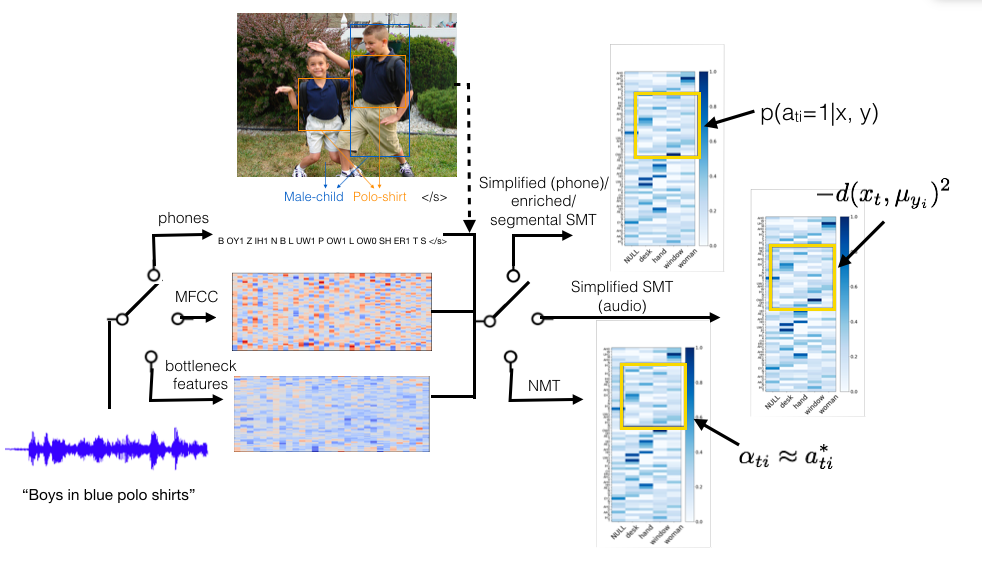
\includegraphics[width=0.8\textwidth]{fig_1.png}
    \caption{Comparison of various multimodal word discovery systems.}
    \label{fig:model_comparison}
\end{figure*}

\subsection{Multimodal image retrieval}
In a standard multimodal image retrieval problem \cite{Karpathy14}, we have a database with image-caption pairs $(\mathbf x^1, \mathbf y^{\pi(1)}), \ldots, (\mathbf x^S, \mathbf y^{\pi(S)})$, where image $\mathbf y^{\pi(i)}$ is uniquely described by sentence $\mathbf x^i$ and vice versa. The goal is to learn the one-to-one mapping $\pi: \{1, \ldots, S\} \rightarrow \{1, \ldots, S\}$ that maps between the indices of each caption to the corresponding image. 

\section{Simplified mixture multimodal alignment models}
At the first glance, Eq. (\ref{eq:smt_trans_prob}) may seem daunting to learn since it contains the summation of $T_x^{T_y+1}$ terms and can be hard to break down into a reasonable amounts of parameters. However, if each feature frame is assumed to be independently generated by a single concept selected uniformly from the set of image concepts, the expression can be broken nicely into the translation probabilities between single pairs of concepts and acoustic frames/phonetic label. Such a model is referred later as \textit{simplified mixture models}.
%is simply the likelihood of the audio feature given the image concept and alignment, which can be modeled frame-wise as a mixture distribution. Such a model is referred  as \textit{simplified mixture models}. 

\subsection{Phone-level model}
 For the phone-level word discovery, following \cite{Brown92}, we can make use of the following assumptions:
\begin{enumerate}
    \item \textit{Hard alignment assumption}: $\mathbf{A}$ is integer-valued, specifically $A_{it}=1$ for $i=i(t)$, else $a_{it}=0$;
    \item \textit{Uniform prior assumption}: all alignments are equally likely given only $\mathbf{y}$: $p(\mathbf A|\mathbf y) = \frac{\epsilon}{(T_y+1)^{T_x}}$, where $\epsilon$ is some normalization constant;
    \item \textit{Mixture assumption}: given the alignment,
%$\forall y_j, j\neq a_i$ is conditionally independent of $x_i$ and $x_i$'s are independent of $x_j, j\neq i$ given $y_{a_i}$:$p( \mathbf{x}|\mathbf{y}, \mathbf{a}) = \prod_{i=1}^{T_x} p(x_i|x_{1:i-1}, y_{a_i}) = p(x_i|y_{a_i})$.
each phone depends only on its aligned image concept, thus
$p(x_t|x_{1:(t-1)},\mathbf{A},\mathbf{y})=p(x_t|y_{i(t)})$,
\end{enumerate}
Eq. (\ref{eq:smt_trans_prob}) is then simplified to:
\begin{align}
%    &\frac{\epsilon}{(T_y+1)^{T_x}}\sum_{a_1 = 0}^{T_y} \sum_{a_2 = 0}^{T_y}\ldots \sum_{a_{T_x} = 0}^{T_y} 
%    \prod_{i=n}^{T_x}p(x_i|y_{a_i}).
    &\frac{\epsilon}{(T_y+1)^{T_x}}\prod_{t=1}^{T_x}\sum_{i(t)=0}^{T_y} p(x_t|y_{i(t)}).
\end{align}
Model under such assumptions are called \textit{mixture model} mainly due to the independence between alignments. Optimization with EM results in 
%which can be optimized with EM algorithm and result in
an iterative formula
in terms of the expected counts of a given phone-concept pattern \cite{Brown93}:
\begin{align}
\label{eq:expected_count_ibm1}
    \langle c(x_t|y_i;\mathbf x, \mathbf y)\rangle = \frac{p(x_t|y_i)}{\sum_{i'=1}^{T_y}p(x_t|y_{i'})}.
\end{align}

The optimal alignment between the phones and image concepts can be then obtained by finding the highest-scored translation pair of a given sentence:
\begin{align}\label{eq:smt_alignment}
    i^*(t) = \arg\max_i p(x_t|y_i).
\end{align}

\subsection{Audio-level model}
To deal with continuous acoustic features, it is natural to apply
KMeans-based clustering algorithm and model each image concept $y_i$ as a set of clusters with centroid $\{\mu_{y_i}^m\}_{i=1, m=1}^{T_y, M}$. Intuitively, it is clear that one image concept should be associated with more than one cluster since words in general consists of more than one phone or syllable, and even feature for one phone may require more than one cluster to model due to the variation of the speech production process. Instead of maximizing the likelihood function, the model tries to minimize:
\begin{align}\label{eq:multimodal_kmeans_obj}
    \min_{\mathbf A \in \mathcal A, \mathbf m \in [M]^{T_x}} \sum_{t=1}^{T_x} \|x_t - \mu_{m(t)}(y_{i(t)})\|^2_2,
\end{align}
the update is similar to the standard KMeans algorithm but guided by the image concepts corresponding to each utterances:
\begin{align}\label{eq:multimodal_kmeans_update}
    &i^*(t), m^*(t) = \arg\min_{i, m}\|x_t - \mu_m(y_{i})\|^2\\
    &\mu_m(y_i) = \frac{\sum_{t: i(t)=i, m(t)=m} x_t}{c(i, m;\mathbf x, \mathbf y)}.
\end{align}

% needed in second column of first page if using \IEEEpubid
%\IEEEpubidadjcol

\section{Enriched mixture multimodal alignment models}
\subsection{Phone-level model}
% IBM 2
\cite{Brown92} has proposed several extensions to the phone-level simplified mixture model. One extension is to relax the uniform prior assumption by making the alignment probability time-dependent. Specifically they introduce a set of parameters $p(i|t, T_x, T_y) := \mathbf{Pr}[i(t) = i|\mathbf x_{1:t}, \mathbf y_{1:i}, T_x, T_y], i\in \{1,\ldots,T_y\}, t\in \{1,\ldots,T_x\}$ with the constraint that $\sum_{i=0}^{T_y} p(i|t, T_x, T_y) = 1$. This time-dependent alignment is capable of capturing the property that the feature frames aligned to a image concept tend to be in similar order and position as the image concept. As a result, Eq. (\ref{eq:smt_trans_prob}) is modified to be:
\begin{align}
    \frac{\epsilon}{(T_y+1)^{T_x}}\prod_{t=1}^{T_x} \sum_{i(t)=0}^{T_y}p(i(t)|t, T_x, T_y) p(x_t|y_{i(t)}),
\end{align}
The expected count is then a weighted version of the simplified mixture counterpart:
\begin{align}
\label{eq:expected_count_ibm2}
    \langle c(x_t|y_i; \mathbf x, \mathbf y) \rangle = \frac{p(i|t, T_x, T_y) p(x_t|y_i)}{\sum_{i'=1}^{T_y}p(i'|t, T_x, T_y) p(x_t|y_{i'})}.
\end{align}

% discuss more about IBM 3, 4, 5 

\subsection{Audio-level model}
 % Continuous IBM model
The audio-level SMA models is similar to the phone-level mixture model, except a continuous mixture distribution is used to model the common phone-like units associated with each concept. For example, a Gaussian mixture model (GMM) can be used to model each image concept:
\begin{align}\label{eq:gmm_prob}
    p(x_t|y_i) = \sum_{m=1}^{M} c_m(y_i) N( x_t|\mu_m(y_j), \Sigma_m(y_j)),
\end{align}
where $\{c_m(y)\}_{i=1}^M$ is the prior distribution for each mixture associated with concept $y_i$. Under the same assumption (1)-(3) as the discrete mixture model, the expected count of the continuous mixture model takes the form:
%\begin{align}\label{eq:gmm_prob}
%    p(\mathbf x|\mathbf y, \mathbf A) &= \frac{\epsilon}{(T_y+1)^{T_x}}\prod_{t=1}^{T_x}\sum_{m(t)=1}^{M} c_{m(t)}(y_{i(t)})\nonumber\\
%    &\mathcal{N}(\mathbf x_t|\mu_{m(t)}(y_{i(t)}), \Sigma_{m(t)}(y_{i(t)})).
%\end{align}
% GMM model
%\begin{align}\label{eq:cont_gmm_em_update}
%    \hat c_m(i) &= \frac{\sum_{t=1}^{T_x}\gamma_t(i, m)}{\sum_{t=1}^{T_x}\sum_{m=1}^{M}\gamma_t(i, m)}\\
%    \hat \mu_m(y_i) &= \frac{\sum_{t=1}^{T_x}\gamma_t(i, m)x_t}{\sum_{t=1}^{T_x}\sum_{m=1}^{M}\gamma_t(i, m)}\\
%    \hat \Sigma_m(y_i) &= 
%    \frac{\sum_{t=1}^{T_x}\gamma_t(i, m)(x_t - \mathbf \mu_m(y_i))(x_t - \mathbf \mu_m(y_i))^\top}{\sum_{t=1}^{T_x}\sum_{m=1}^{M}\gamma_t(i, m)}.
%\end{align}
\begin{align}\label{eq:expected_count_gmm}
    &\langle c_t(i, m;\mathbf x, \mathbf y) \rangle =\nonumber\\ &\frac{c_{m}(y_{i})N(\mathbf x_t|\mu_{m}(y_{i}), \Sigma_{m}(y_{i}))}{\sum_{i'=1}^{T_y} \sum_{m=1}^M c_m(y_{i'})N(\mathbf x_t|\mu_m(y_{i'}), \Sigma_m(y_{i'}))} \\
    &\langle c_t(x_t|y_{i}; \mathbf x, \mathbf y) \rangle = \sum_{m=1}^M \langle c_t(i, m; \mathbf x, \mathbf y) \rangle.
\end{align}

EM algorithm for GMM tries to maximize the \textit{Baum auxiliary function}:
\begin{align}\label{eq:multimodal_gmm_objective}
&Q(\bar{\Theta}, \Theta) = \sum_{t=1}^{T_x}\sum_{i(t)=0}^{T_y}\sum_{m(t)=1}^M p(i(t), m(t)|\mathbf x, \mathbf y, \bar {\Theta}) \cdot \nonumber\\
&\log p(x_t, i(t), m(t)| \mathbf y, \Theta)
%&= \sum_{t=1}^{T_x}\sum_{i(t)=0}^{T_y}\sum_{z_t=1}^M p(i(t), m(t)|\mathbf x_t, \mathbf y, \bar{\Theta}) \nonumber\\
%&(-\frac{1}{2}\log (2\pi)^d|\Sigma_{m}(y_i)| + 
%\log c_{m(t)}(y_{i(t)}) - \nonumber \\
%&\frac{1}{2} (\mathbf{x}_t - \mathbf \mu_{m}(y_{i(t)}))^{\top}\Sigma_m(y_{i(t)})^{-1}(\mathbf{x}_t - \mathbf \mu_{m}(y_{i(t)}))).
\end{align}
Although not the logarithm of the translation probability as in the discrete case, this auxiliary function is know to provide a lower bound for the log-translation probability and guarantees to converge to a local optimum \cite{Bilmes1998}. The main advantage of using Baum auxiliary objective is that the mixture means and variances now have closed-form expressions in term of the expected count and the acoustic feature frames. The auxiliary function approach will be applicable to all the audio-level SMA models with continuous features in the subsequent sections. More details about the EM update with Baum auxiliary function can be found, for example, in \cite{Bilmes1998}. 
%Further, similar to the discrete case, the model keeps track of the expected counts $\gamma_t(i, m) := p(i(t)=i, z_t=m|\mathbf x, \mathbf y, \bar \Theta)$ and the mixture priors, means and variance of the GMM are updated as follows: 

In fact, the KMeans-based algorithm in the previous section can be seen as a simplification of the enriched mixture model when the mixture distribution is a Gaussian mixture with diagonal and asymptotically zero covariances for each component. 
%The continuous HMM model can be similarly derived from the discrete one with an GMM as the emission probability for each image concept. 


%\section{Audio-level multimodal word discovery}
%A next essential step is to model the probability distribution of the acoustic vectors. There are again two alternatives: One is to approximate the density function by a mass function by clustering the acoustic features into discrete units; the other is to learn the continuous distribution directly. The second approach is more theoretically sound and thus will be the focus of this paper. It turns out that the second approach allows a natural extension of both the statistical models \cite{Brown92} and neural models \cite{Bahdanau14} to model problems where the source language is continuous, as in the case of multimodal acoustic word-unit discovery and speech-to-translation.

\section{Segmental multimodal alignment models}
\begin{figure*}[t]
    \centering
    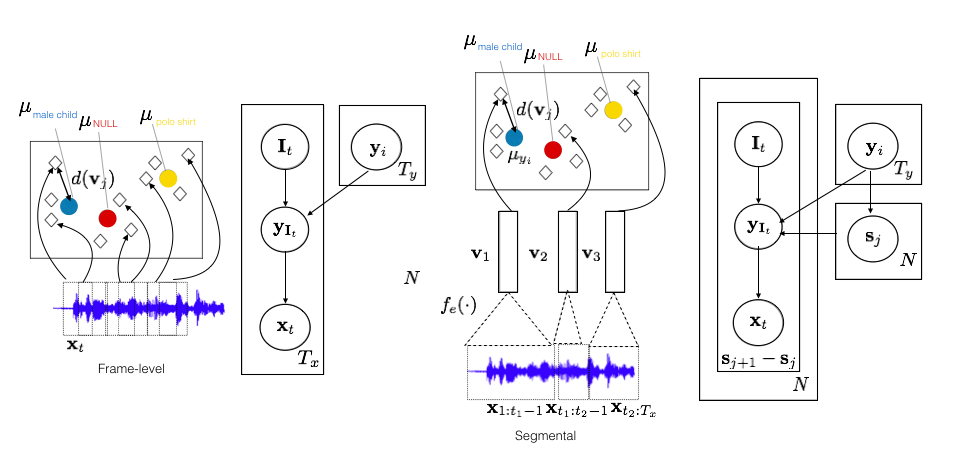
\includegraphics[width=0.8\textwidth]{fig_2.png}
    \caption{Framewise model vs. segmental model}
    \label{fig:frame-segmental-comparison}
\end{figure*}
One major bottleneck of performance for mixture models is its independence assumption. The alignments for each feature frames are assumed to be independent and thus the global patterns formed by multiple acoustic feature frames is overlooked. As a result, each feature frames need to  combine enough context of the original speech waveform in order to well represent a word-like unit. However, such an assumption fails to hold for acoustic features like MFCC and even bottleneck features although the latter is known to be good at compressing the contextual information within individual frame. Another problem is that the mixture assumption will make the phone sequence of any arbitrary order to have the same probability. In the phone-level discovery case, the word ``god'' and ``dog'' will have the same probability for two completely different image concepts. One natural approach to capture the multi-frame patterns is to replace the framewise model with an acoustic model that operates at the level of \textit{segment} \cite{Kamper2017}. A segment is defined in this context as a variable-length sequence of consecutive audio feature frames that potentially represent a word or subword unit. This class of models is referred as \textit{segmental models}.   

%Another problem is that the mixture assumption will make the phone sequence of any arbitrary order to have the same probability. In the phone-level discovery case, the word ``god'' and ``dog'' will have the same probability given an image concept; in the audio-level case, things get worse especially when using MFCC as the feature as a single feature frame of two different words may be very similar and too local to discriminate the words. Another issue is that the independence assumption tends to make the alignment ``fragmental'' since it fails to account for the fact that sequences nearby are more likely to align to the same object. In other words, a better model should take into account the conditional dependence between alignments and the fact that speech is more naturally modelled as a sequence of \textit{segments}, which is defined as a variable-length sequence of consecutive audio feature frames that potentially represent a word, rather than simply a sequence of frames. This class of models is referred as \textit{segmental models} \cite{Kamper2016, Kamper2016}. 

\subsection{Phone-level word discovery}
% HMM model
On the phone-level, since most words do not have more than four syllables the segments can be modeled as the local dependence between alignments. We may replace the uniform prior assumption with the following \textit{Markov assumptions}: $p(i(t)|i(1:t), T_y) =: p(i(t)|i(t-1), T_y)$. Eq. (\ref{eq:smt_trans_prob}) then simplifies to:
\begin{align}\label{eq:trans_prob_hmm}
    p(\mathbf x|\mathbf y) &= \frac{\epsilon}{(T_y+1)^{T_x}}\sum_{\mathbf A \in \mathcal A}\prod_{t=1}^{T_x} p(i(t)|i(t-1), T_y) p(x_{t}|y_{i(t)}),
\end{align}
where $p(i(1)|i(0)) = p(i(1))$. This model, as first shown by \cite{Vogel1996, Och2003}, is a hidden Markov model (HMM) with alignment vectors as the states. Maximizing Eq. (\ref{eq:trans_prob_hmm}) amounts to collect the expected counts:
\begin{align}\label{eq:expected_counts_dhmm}
\langle &c(i(t-1), i(t)|\mathbf x, \mathbf y)\rangle
= \nonumber\\
&\frac{\alpha_{t-1}(i(t-1))p(i(t)|i(t-1), T_y)p(x_t|y_{i(t)})\beta_{t}(i(t))}{\sum_{i=1}^{T_y}\alpha_{t-1}(i(t-1))p(i|i(t-1), T_y)p(x_t|y_{i})\beta_t(i)}\\
&\langle c(x_t|y_i; \mathbf x, \mathbf y)\rangle
= \sum_{i'=1}^{T_y}\langle c_t(i', i| \mathbf x, \mathbf y)\rangle,
\end{align}
where $\alpha_t(i) := p(x_{1:t}, i(t)=i|\mathbf y)$ and $\beta_t(i) := p(x_{t+1:T_x}|i(t)=i, \mathbf y)$ can be updated iteratively via dynamic programming.


% Therefore, following \cite{Vogel1996}, we introduce the parameters $\pi(i|T_y) \approx p(\mathbf a_{1, i}=1|T_y)$ and $r(|j-i||T_y) \approx p(\mathbf a_{t,j}=1|\mathbf a_{t-1, i}=1, T_y)$, subject to the constraints that $\sum_{k=1}^{T_y}\pi(k) = 1, \sum_{k=0}^{T_y-1} r(k|T_x, T_y) = 1$, which can be treated as the initial and transition probabilities of a Markov chain. Eq. The model then again tries to maximize 

%Plug Eq. (\ref{eq:align_prob_hmm}) into Eq. (\ref{eq:smt_trans_prob}) and apply standard forward-backward algorithm for HMM \cite{Rabiner89-ATO}, it can be shown that:
%\begin{align}
%\label{eq:dhmm_em_update}
%    \hat p(i) &= \frac{\sum_{t=1}^{T_x}\alpha_t(i)\beta_t(i)}{\sum_{t=1}^{T_x}\sum_{i=1}^{T_y}\alpha_t(i)\beta_t(i)}\\
%    \hat p(j|i, T_y) &=  \frac{\sum_{t=1}^{T_x}\alpha_t(i)p(j|i, T_y)p(x_{t+1}|y_{i(t+1)})\beta_t(i)}{\sum_{t=1}^{T_x}\sum_{i=1}^{T_y}\alpha_t(i)p(j|i, T_y)p(x_{t+1}|y_{i(t+1)})\beta_t(j)}\\
%    \hat p(x_t|y_i) &= \frac{\sum_{t=1}^{T_x}\gamma_t(i)}{\sum_{t=1}^{T_x}\sum_{i'=1}^{T_y}\gamma_t(i')},
%\end{align}
%for all $t \in \{1, \cdots, T_x\}, i, j \in \{1, \cdots, T_y\}$ and all pairs of phonemes and concepts, where $\alpha_t(i) := p(\mathbf x_{1:t}, i(t)=i|\mathbf y)$, $\beta_t(i) := p(\mathbf x_{t+1:T_x}| i(t)=i)$. $\gamma_t(i) := p(\mathbf x, i(t)=i|\mathbf y) = \alpha_t(i) \beta_t(i)$ is the expected count for the alignment at time $t$ to concept $i$. One simplification of the model mentioned in \cite{Vogel1996} is to add the constraint that $p(j|i, T_y) = q(j-i|T_y)$ since the alignment of the current state depends only on the relative change of aligned position with respect to the previous alignment. For multimodal word discovery, since the order of the concept does not matter, the number of parameters for the transition probability can be further reduced by $p(j|i, T_y) = q(T_y) \delta_{ij} + (1-q(T_y))(1-\delta_{ij})$, where $\delta_{ij} = 1$ if $i=j$ and 0 otherwise. In other words, the alignment of the current phone depends only on whether it aligns to the same concept as the previous phone or not. 

standard Viterbi decoding can be applied to find the optimal alignment between concept and phone: 
\begin{align}\label{hmm_alignment}
    i^*(t) &= \max_{1 \leq i \leq T_y}\{p(\mathbf x_{1:t-1}, i(1:t-1)|\mathbf y) p(i|i(t-1))p(x_t|y_i)\}.
\end{align}
For the image retrieval, the translation probability from Eq. (\ref{eq:trans_prob_hmm}) is used to find the optimal set of image concepts:
\begin{align*}
    \mathbf y^* &= \max_{\mathbf y} p(\mathbf x|\mathbf y) = \max_{\mathbf y} \sum_{i=1}^{T_y}\alpha_{T_x}(i).
\end{align*}

\subsection{Audio-level word discovery}
While modeling intermediate correlations between alignments may be sufficient for phone-level word discovery, the audio-level feature may require modeling directly on the level of segment. Let $N$ be the number of segments, a \textit{segmentation} is uniquely characterized by the vector $\mathbf s = [s_1, \cdots, s_N]$, where $s_j$ is the starting frame of segment $j$. Assume that the first word starts at the first frame and the last word ends at the last frame, we have $s_1 \equiv 1$, $s_j < s_{j+1}, 1\leq j \leq N$ and $s_{N+1} := T_x+1$. The segmentation can be alternatively represented by a binary \textit{boundary vector} $\mathbf b \in \{0, 1\}^{T_x}$ such that $b_{s_j}=1, j=1,\ldots,N$ and 0 otherwise. Let $\mathcal S_{T_x, N}$ denotes all the segmentation of length N for feature sequence of length $T_x$. By the definition of the segment, all feature frames belonging to the same segment will align to the same image concept. As a result, if the segmentation is known, the alignment matrix $\mathbf A$ can be compressed into a smaller matrix $\tilde{\mathbf{A}} \in \{0, 1\}^{T_y \times N}$ with the property in Eq. (\ref{eq:one-concept-assumption}), which will be referred to as the \textit{assignment matrix}. Let the set of all assignment matrix for $N$ segment be $\tilde{\mathcal A}_N$ the translation probability of the segmental model can be expressed as:
\begin{align}\label{eq:trans_prob_segmental}
    p(\mathbf x|\mathbf y) &= \sum_{N=N_{min}}^{N_{max}} \sum_{\mathbf s \in \mathcal S_N} p(\mathbf s|\mathbf y)\sum_{\tilde{\mathbf{A}} \in \tilde{\mathcal A}_N} p(\tilde{\mathbf{A}}| \mathbf s, \mathbf y) p(\mathbf x|\tilde{\mathbf A}, \mathbf s, \mathbf y).
\end{align}
The expression shows that once the segmentation is fixed, the problem reduces to maximize the likelihood of the segments given the image concept.

Suppose there is a subword-level segmentation $\mathbf s^*$ based on prior knowledge, for instance, the acoustic properties of the syllable units, the problem reduces to maximize:
\begin{align}\label{eq:trans_prob_preseg_simplified}
   p(\mathbf x|\mathbf y) \approx p(\mathbf x|\mathbf y, \mathbf s^*). 
\end{align}
Consequently, with a similar Markov assumption as in the phone-level word discovery, the translation probability can be broken into probabilities of the subword units:
\begin{align*}
    p(\mathbf x|\mathbf y, \mathbf s^*) &= \frac{\epsilon}{(T_y+1)^N}\prod_{j=1}^{N} \sum_{i(j)=0}^{T_y+1}p(i(j)|i(j-1), \mathbf y)\nonumber\\ &p(x_{s_j:s_{j+1}}|y_{i(j)}, m(j))    
\end{align*}
which can be modelled using an HMM with a mixture observation density: $p(x_{s_j:s_{j+1}}|y_{i(j)}) = p(m(j)|y_{i(j)}, \mathbf s) p(x_{s_j:s_{j+1}}|y_{i(j)}, m(j))$. The Baum auxiliary function for the segmental model is then:
\begin{align}\label{eq:baum_subword_hmm}
    %L(\bar{\Theta}, \Theta) &= \sum_{j=1}^{N}\sum_{i(t-1)=0}^{T_y}\sum_{i(t)=0}^{T_y} p(i(j-1), i(j), m(j)|\mathbf x, \mathbf y, \mathbf s^*) \nonumber\\
    &Q(\bar{\Theta}, \Theta) = \nonumber\\
    & \sum_{j=1}^N \mathbb{E}_{\mathbf i, \mathbf m}[\log p(x_{s_j^*:s_{j+1}^*}, i(j), m(j)|i(j-1), y_{i(j)}, \Theta)|\mathbf x, \mathbf y, \bar{\Theta}].
\end{align}
The challenge here is that the segments are variable in lengths and $p(x_{s_j:s_{j+1}}|y_{i(j)})$ can not be directly modelled with a fixed dimensional density function. Besides modeling each segment using HMM \cite{Lee2012}, one existing approach \cite{Kamper2017} is to embed each segment into a fixed-dimensional space as \textit{embedding vector} so the embedding vector can be modelled with a fixed dimensional density function. Denote the embedded $j$-th segment as $\tilde{x}_j = f_e(x_{s_{j-1}:s_j}), s_0:=1$ and $\tilde{\mathbf x} := [\tilde{x}_1, \cdots, \tilde{x}_N]$, the assumption amounts to $p(x_{s_j:s_{j+1}}|y_{i(j)}) p(\tilde{x}_j|y_{i(j)})^{s_{j+1}-s_j}, p(\tilde{x}_j|y_{i(j)}) = \sum_{m=1}^M c_m(y_{i(j)})\mathcal N(\tilde{x}_j|\mu_m(y_{i(j)}), \Sigma_m(y_{i(j)}))$. A special case of such embedding assumption is that most spoken words are distinguisable by the ear even after they are properly scaled to the same size. Therefore, the embedding vector can simply be the resampled version of the segments. While duration carries information in many languages and the embedded segment may suffered from loss of high-frequency information when the downsampling rate is too high, embedding segments to fixed length greatly reduces the complexity of the model. This model is referred later as the \textit{static segmental HMM}.

Suppose $\mathbf s^*$ is instead a word-level pre-segmentation and the pseudo-word segments satisfy the following \textit{segmental mixture assumption}: Given the assignment, each segment depends only on its aligned image concept, thus $p(\mathbf x_{s_j:s_{j+1}-1}|\mathbf x^{-}, \tilde{\mathbf{A}}, \mathbf s, \mathbf y) = p(\tilde{\mathbf x}_j|\mathbf y_{i(s_j)})$, where $\mathbf x^-$ denotes the segments other than $j$. Combined with the embedding vector approach, a simplified or enriched mixture model can be used to model the segments.

The approaches above fixed the noisy word boundaries through the clustering process and its performance is then constrained by the quality of the pre-segmentation. It is more appealing to jointly refine the segmentation and clusters during training \cite{Kamper2017}. Suppose given the segmentation, the utterance can be modeled by an enriched mixture model, then the Baum auxiliary function is:
\begin{align}\label{eq:baum_segmental}
    Q(\bar{\Theta}, \Theta) &= \sum_{N=N_{min}}^{N_{max}}\sum_{\mathbf s \in \mathcal S^N}p(\mathbf s|\mathbf x, \mathbf y, \bar{\Theta})\nonumber\\
    &\mathbb{E}_{\mathbf i, \mathbf m}\left[\log p(\mathbf x, \mathbf s, \mathbf i, \mathbf m|\mathbf y, \mathbf \Theta)|\mathbf x, \mathbf y, \mathbf s , \bar{\Theta}\right].
    %p(i(j), m(j)|\mathbf x, \mathbf y, \mathbf s, \bar{\Theta})\nonumber\\
    %&\mathbb{E}_{\mathbf s}\left[\sum_{j=1}^N\log p(\tilde{\mathbf{x}}, \mathbf s, \tilde{\mathbf A}|\mathbf y, \Theta)|\mathbf x, \mathbf y, \mathbf s, \bar{\Theta}\right].
\end{align}
One key challenge of this approach is to model the distribution of the segmentation $p(\mathbf s|\mathbf x, \mathbf y)$ and $p(\mathbf s|\mathbf y)$. Similar to the prior probabilities of alignments, the summation over the priors and posteriors of segmentation in Eq. (\ref{eq:trans_prob_segmental}) and Eq. (\ref{eq:baum_segmental}) respectively has $(N_{max}-N_{min})\left(\begin{array}{c}
      T_x\\
     N-1
\end{array}\right)$ terms and requires an prohibitive amount of parameters. Suppose $p(\mathbf s|\mathbf x, \mathbf y)$ and $p(\mathbf s|\mathbf y)$ are known, we can approximate the sums by its unbiased sampled version:
\begin{align}\label{eq:baum-besgmm-sampled}
    p(\mathbf x|\mathbf y) &\approx p(\mathbf x|\mathbf y, \mathbf s')\\
    Q(\bar{\Theta}, \Theta) &\approx \mathbb{E}_{\mathbf s}\left[\log p(\tilde{\mathbf x}, \mathbf s'')|\mathbf y|\mathbf x, \mathbf y, \mathbf s'', \bar{\Theta}\right],
\end{align}
where $\mathbf s' \sim p(\mathbf s|\mathbf y), \mathbf s'' \sim p(\mathbf s|\mathbf x, \mathbf y)$. Notice that this expressions are the same as those of the models with fixed segmentation, except the segmentations are now drawn randomly rather than deterministically.

To model $p(\mathbf s|\mathbf x, \mathbf y)$ and $p(\mathbf s|\mathbf y)$, One approach 
 is to use \textit{adaptor grammar}\cite{Johnson2007, Lee2012}, which assumes the segmentation boundary vector $\mathbf{b}$ to be a sequence of i.i.d Bernoulli random variables with parameter $\alpha_b$. $\alpha_b$ is assumed to be generated by a symmetric Dirichlet process to encourage sparsity of the boundary vector. During inference, the boundary vector and Bernoulli parameter can be sampled efficiently using a collapsed Gibbs sampler. Once the boundary vector is fixed, each segment can be modelled separately. The second approach is employed by the BES-GMM system \cite{Kamper2017} and assumes each segmentation $s_j$ to be uniformly distributed between $[0, s_{j+1}]$. Under this assumption and the segmental mixture assumption, $\mathbf s$ can be sampled backward from the posterior $p(\mathbf s|\mathbf x, \mathbf y)$:
 \begin{align*}
     s_j &\sim p(s_j|\mathbf s_{-j}, \mathbf x, \mathbf y)\\
     &\propto p(s_j, s_{j+1}, \mathbf x_{1:s_{j+1}}|\mathbf y)\\
     &\propto p(\mathbf x_{1:s_{j+1}}|s_j, s_{j+1}, \mathbf y) p(|\mathbf y)\\
     &\propto p(\mathbf x_{1:s_{j}}|\mathbf y) p(\tilde{x}_j|\mathbf y)^{(s_{j+1}-s_j)},
 \end{align*}
 where the second $\propto$ uses the uniform assumption of $s_j$. $p(\mathbf x_{1:s_{j}}|\mathbf y)$ can be computed recursively with dynamic programming. Optimizing Eq. (\ref{eq:baum-besgmm-sampled}) with EM algorithm results in a formula in terms of the following expected count:
 \begin{align}\label{eq:expected_counts_besgmm}
     &\langle c_j(i, m;\mathbf s, \mathbf x, \mathbf y)\rangle\\
     &= \frac{(c_{m}(y_{i})\mathcal N(\tilde{x}_j|\mu_{m}(y_{i}), \Sigma_{m}(y_{i})))^{s_{j+1}-s_j}}{\sum_{i=0}^{T_y}\sum_{m=1}^M (c_{m}(y_{i})\mathcal N(\tilde{x}_j|\mu_{m}(y_{i}), \Sigma_{m}(y_{i})))^{s_{j+1}-s_j}}.
 \end{align}
 
 The model infers the optimal segmentation and alignment using Viterbi decoding:
\begin{align}\label{eq:decode_besgmm}
    s_j^*, i^*(j) &= \max_{s_j, i}\{p(\mathbf x_{1:s_j}|y_{i})p(\tilde{x}_j|y_{i})^{s_{j+1}-s_j}\},
\end{align}
where similar to the sampling step, the $p(\mathbf x_{1:s_j}|y_{i})$ is evaluated forward from $s_j=1$ while the optimization starts from backward from $s_{j+1}=T_x+1$. This model is based on BES-GMM \cite{Kamper2017} with additional image concepts input and referred later as dynamic segmental model. When the segmentation is fixed during training, the model is referred as static segmental GMM. \cite{Kamper2017} also proposes a simplified version of the BES -GMM called ES-KMeans, which can be naturally adapted to the multimodal setting to optimize:
\begin{align}\label{eq:objective_multimodal_eskmeans}
    \min_{\mathbf s, \mathbf A, \mathbf m}\sum_{j=1}^{N}(s_j-s_{j-1})\|v_j - \mu_{m(j)}(y_i(j))\|_2^2.
\end{align}
This simplified model is referred later as simplified dynamic segmental model.

\section{NMA models}
Similar to the SMA model, the NMA makes use of several assumptions:
\begin{enumerate}
    \item \textit{Dominant path assumption}: There is a ``dominant'' alignment $\mathbf A^*$ such that $p(\mathbf A^*|\mathbf x) \approx 1$;
    \item \textit{Embedding assumption}: The input representation of the phone $x_t$ can be compressed into a lower-dimensional embedding $h_t(x_t) =: \mathbf h_t$, $\forall t \in \{1, \cdots, T_x\}$. Let $\mathbf h = [\mathbf h_1, \cdots, \mathbf h_{T_x}]$;
    \item There exists some ``context'' vector $\mathbf c_i(\mathbf h, A^*), i=\{1, \cdots, T_y\}$ such that $y_i$ is conditionally independent of $\mathbf h$ given $\mathbf c_i$.
    \item There exists some ``state'' vector $\mathbf s_i(\mathbf y_{1:i-1})$ such that $y_i$ is independent of $\mathbf y_{1:i-2}$ given $\mathbf s_i$ and $y_{i-1}$.
\end{enumerate}
The dominant path assumption is in stark contrast to the uniform prior assumption of the SMA model and instead of summing over all possible alignments, only a single soft alignment is used to compute the probability. 

By sequentially applying the assumptions above, Eq. (\ref{eq:nmt_trans_prob}) is then simplified to one term:
\begin{align}\label{eq:nmt_trans_prob_simplify}
    p(\mathbf y|\mathbf x, \mathbf A)&= \prod_{i=1}^{T_y} p(y_i|y_{1:i-1}, \mathbf{x}, \mathbf{A}^*) = \prod_{i=1}^{T_y} p(y_i|\mathbf y_{1:i-1}, \mathbf h, \mathbf{A}^*)\\
    &= \prod_{i=1}^{T_y} p(y_i|\mathbf y_{1:i-1}, \mathbf c_i)\\
    &= \prod_{i=1}^{T_y} p(y_i|y_{i-1}, \mathbf s_i, \mathbf c_i).
\end{align}
In the standard attention \cite{Bahdanau14}, the dominant alignment is learned via a soft alignment:
\begin{align}\label{eq:def_soft_align}
    A_{it}:= \alpha_{it} &= \frac{\exp(e(\mathbf h(\mathbf x_t), \mathbf y_i)/T)}{\sum_{j=1}^{T_y} \exp(e(\mathbf h(\mathbf{x}_t), \mathbf y_j)/T)}
\end{align}
where $\mathbf e(\cdot)$ can be learned by a feedforward neural network. Compared to the original attention mechanism, our attention has two main differences: First, the attention weights are normalized across concepts for a given acoustic feature frame; second, the decoder state is not fed into the attention to avoid the dependency of the future states when computing the softmax over all the image concepts. The softmax ensures Eq. (\ref{eq:one-concept-assumption}) is satisfied and $T$ is a temperature term to smooth the softmax. Notice that the original attention can be used while fulfilling the many-to-one assumption if the network learns $p(\mathbf x|\mathbf y, \mathbf A)$ instead. However, such modeling choice is at odds with the discriminative nature of the NMA model: the acoustic features can be  continuous and cannot be divided into a finite number of categories, and thus the output probability cannot be modelled by a softmax function. The context vectors are then learned by:
\begin{align}\label{eq:def_context_vec}
    \mathbf c_i = \sum_{t=1}^{T_x} \alpha_{it}^* \mathbf h_t.
\end{align}
The assumption (3) of this section can be viewed as a soft version of the SMA assumption (3) in the previous section:  in the SMA model, concept $y_i$ depends only on the phones that align to it, which is equivalent to the special case when $\alpha_{it}^*$ in Eq. (\ref{eq:def_context_vec}) is either 0 or 1. Therefore, the set of probabilities $\{p(y_i|y_{i-1}, \mathbf s_{i-1}, \mathbf c_i)\}_{i=1}^{T_y}$ can be learned using a recurrent neural net $f$ with state vector $s_i$. The problem then boils down to learning the functions $h, e, f$ such that the log-likelihood of the concepts given the phone sequence is maximized.

%For the multimodal word discovery model, special modification can be made on the attention mechanism. One way is to notice that since the order of the image concepts do not matter, the recurrent connection can simply be removed and the 
% Talk about the modification on the standard encoder-decoder framework

\section{Experiments}
\subsection{Datasets}
Our dataset consists of 7996 images that are present in the Flickr8k and Flickr30k corpus. We choose to use Flickr8k primary because it contains phrases that describe particular regions of the image, for instance, ``a girl in a pink dress''. The phrase-level segmentation is used as our gold alignment. We only used images that appeared in the Flickr8k dataset so that we can compare our results to the speech-to-image \cite{Harwath15} and text-to-image \cite{Karpathy15} system. In order to make sure that we used the same dataset as in \cite{Karpathy15, Harwath15}, we divided the data into training set (6996 images) and test set (the same 1000 images used in \cite{Karpathy15, Harwath15}).  We use Flickr30kEntities to extract image concepts from the phrase-level descriptions and merged similar entities using WordNet (cite needed) synsets. By considering captions in which every concepts appear at least 10 times, we are able to find a list of 1547 concepts. Repeated concepts in a sentence are merged to maintain the many-to-one mapping between the phone sequence and the image concepts. To generate the phone sequence for the caption, we used CMU dictionary  which consists of 39 distinct phone labels and 69 tokens in total with the stress symbols. Words such as compound words like ``skateboarder'' does not have an entry in the dictionary, we simply replaced it with an \texttt{UNK} symbol. For audio-level discovery, we used audio from Flickr-audio dataset \cite{Harwath15}, which are spoken captions for Flikcr8k collected on Amazon Mechanical Turk. We extract the MFCC feature as in \cite{Rasanen2015, Kamper2016} with 12 cepstral coefficients, 25 ms window and 10 ms overlaps, and normalize it across speakers with cepstral mean variance normalization (CMVN). Another acoustic feature we use is the multilingual bottleneck feature from the BUT project  trained on 20 different languages \cite{Fer2017}. Features longer than 2000 frames are truncated. Using word-level forced alignment by an ASR system (cite needed), we are able to convert the phone-level gold alignment to the alignment of acoustic feature frames. Many of the audio are corrupted and did not have a forced alignments, so we filter them out from our dataset and leave with 6610 images. 
 
\subsection{Evaluation metrics}
% Accuracy, Recall, Precision, F-score
For word-discovery task, we evaluate our systems by comparing the predicted and gold alignments. The \textit{accuracy} is defined as the percentage of phones that align to the correct image concept. To visualize the effects between true positive rate and false positive rate, we plot the receiver operating characteristic (ROC) using the alignment probabilities for SMT and normalized attention weights for NMT. The ROC are defined by treating the word discovery as a retrieval problem, where every image concept is a query and every phone/acoustic feature frame as document. In addition, we use the \textit{recall}, \textit{precision} and \textit{F-score}. Since our dataset is not balanced, the retrieval-based metrics help us to fairly evaluate our systems. For the speech-to-image retrieval task, we follow \cite{Harwath15, Karpathy15} to use recall@1, 5, 10 to measure the performance of our system. We assume a one-to-one mappings between image and caption, despite having a large number of image-caption pairs with similar concepts.      

\subsection{Model parameters}
% Phone-level parameters
% SMT
The main parameters of the phone-level SMT is the translation probabilities and alignment probabilities. We run the simplified mixture model until convergence and the enriched and segmental model for 50 iterations. We initialize $p(x_t|y_i)$ by adding one to the numerator when phone $x_t$ and $y_i$ co-occur in a sentence. For segmental model, we initialize alignment transition matrix with a uniform distribution for each row. 
%Further, we found an empirical improvement on F1 score and accuracy for the segmental model when the translation probability is updated via:
%\begin{align*}
%    \hat{p}(x_t|y_i) = \frac{\sum_{t=1}^{T_x}\gamma_t(i)p(x_t|y_i)}{\sum_{t=1}^{T_x}\sum_{i'=1}^{T_y}\gamma_t(i')p(x_t|y_i)},
%\end{align*}
%rather than the correct formula in Eq. (\ref{eq:dhmm_em_update}). 
%This modified formula turns out to generate alignments somewhere in between the mixture model and the segmental model, thus avoiding many false discoveries suffered by the segmental model. The word discovery result is reported with this modification. But we sticked to the original model for the attention plot and retrieval results. % A more theoretically sound modification of the NULL probability can be found in \cite{Toutanova2002}.

% NMT (including decoding)
For the NMT system, we used a 512-dimensional embedding layer followed by a single layer bidirectional LSTM with 512 hidden nodes as the encoder and another single layer LSTM with 512 hidden nodes as decoder. % Confirm needed for the type of initialization
%For the decoding, we rescale the attention weights by its prior probability, which approximately converts the posterior probability to the likelihood, provided the observation has uniform prior: 
%$$
%\frac{p(y_i|x_t)}{p(y_i)} \propto \frac{p(y_i|x_t)p(x_t)}{p(y_i)} = p(x_t|y_i)
%$$. 

% Audio-level parameters
For audio-level simplified mixture model, the main hyperparameter is the number of mixtures per concept $M$ and the dimension of the acoustic embedding. We found that $M=5$ produces the best results and any value larger than 5 leads to many empty clusters. For the enriched mixture model, the covariance matrices become singular as the posterior of certain mixture becomes too small, so we simply fix it to be $0.002$ for the framewise approach and $2$ for the pre-segmental approach, based on the increase of log-likelihood during training. Both models are initialized with randomly generated clusters and assignments. For the segmental model, we used $M=1$ for computational efficiency and initialized the cluster randomly. For the embedding dimension, we experimented with 10 and 20 equally spaced frames and found only marginal improvement when using 20 equally spaced frames  with proper resampling or interpolation, so we follow \cite{Kamper2017} to concatenate 10 equally spaced frames. 
Again following \cite{Kamper2016}, we pre-segmented the audio to syllable-level using the unsupervised syllable-segmentation system by \cite{Rasanen2015} and only consider the boundaries detected by the system during the segment step. This limits the performance of our system to the coverage of their system, but significantly reduces the disk space for storing the embeddings and inference time. To ensure a better coverage of the true word boundaries, we combine the landmarks detected by all three syllable segmentation algorithms (Oscillator, EnvMin, VSeg) \cite{Rasanen2015} and remove boundaries that are within 20 ms from each other. This results in a coverage of about $83.5 \%$ of all the word boundaries to be within 30 ms. Due to run time constraint, we experiment mainly with the ES-Kmeans based segmental system and leaves the comparison with BES-GMM for future work. From our preliminary experiments, the word segmentation results of the two models are very similar.
% What is the exact coverage of the system?

\subsection{Results}
\subsubsection{Phone-level discovery}
\begin{table}[t]
    \centering
    \begin{tabular}{|c|c|c|c|c|}
\hline
        & \begin{tabular}{@{}c@{}}
     Simplified \\
     Mixture
\end{tabular} & \begin{tabular}{@{}c@{}}
     Enriched \\
     Mixture
\end{tabular} & \begin{tabular}{@{}c@{}}
     Segmental\\
     (HMM)
\end{tabular} & NMT \\
        \hline
Accuracy & 43.8 &   40.0    & \textbf{55.4}  & 41.5\\

Recall  & 52.9   &  46.9 & \textbf{67.4} & 29.2\\

Precision   & 46.7  & 41.4  & \textbf{56.7}  & 33.0  \\

F1  & 49.6  & 44.0  & \textbf{61.6}  & 31.2  \\
\hline
\begin{tabular}{@{}c@{}}
     Avg. Word Length \\
     (True Avg. = 9.13)
\end{tabular} & 2.58  & 2.62 & \textbf{6.88} & 20.7
\\
\hline
\end{tabular}
    \caption{Phone-level Word Discovery Results}
    \label{tab:phone_level_result}
\end{table}
\begin{figure*}[t]
    \centering
    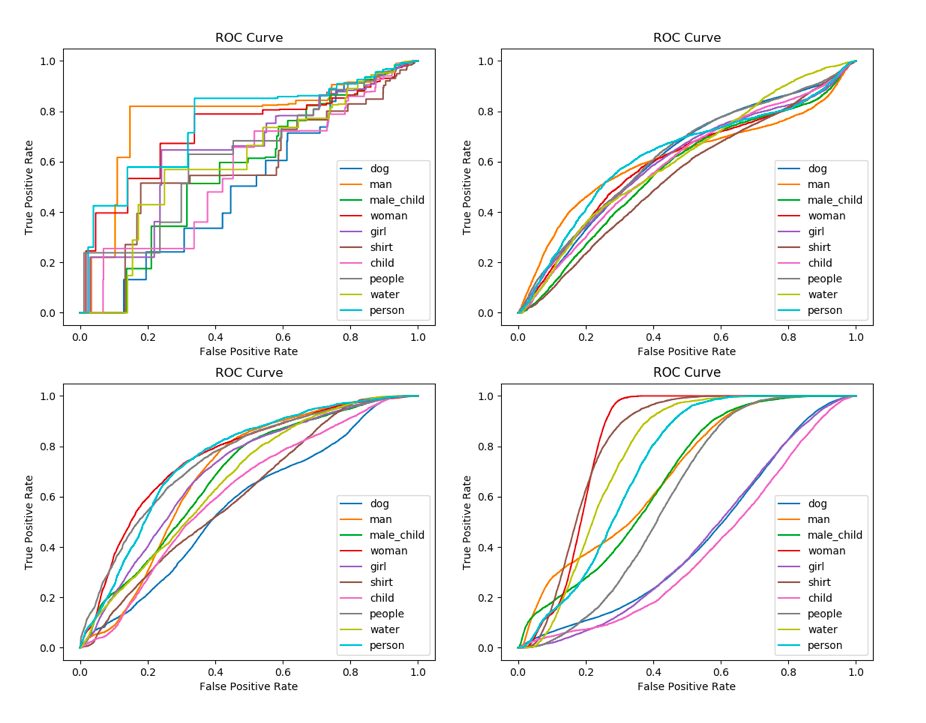
\includegraphics[width=0.8\textwidth]{fig_3.png}
    \caption{ROC for phone-level models. Top-left: the simplified mixture model; top-right: the enriched mixture model; bottom-left: the segmenal model; bottom-right: NMT}
    \label{fig:roc_phn}
\end{figure*}

\begin{figure*}[t]
    \centering
    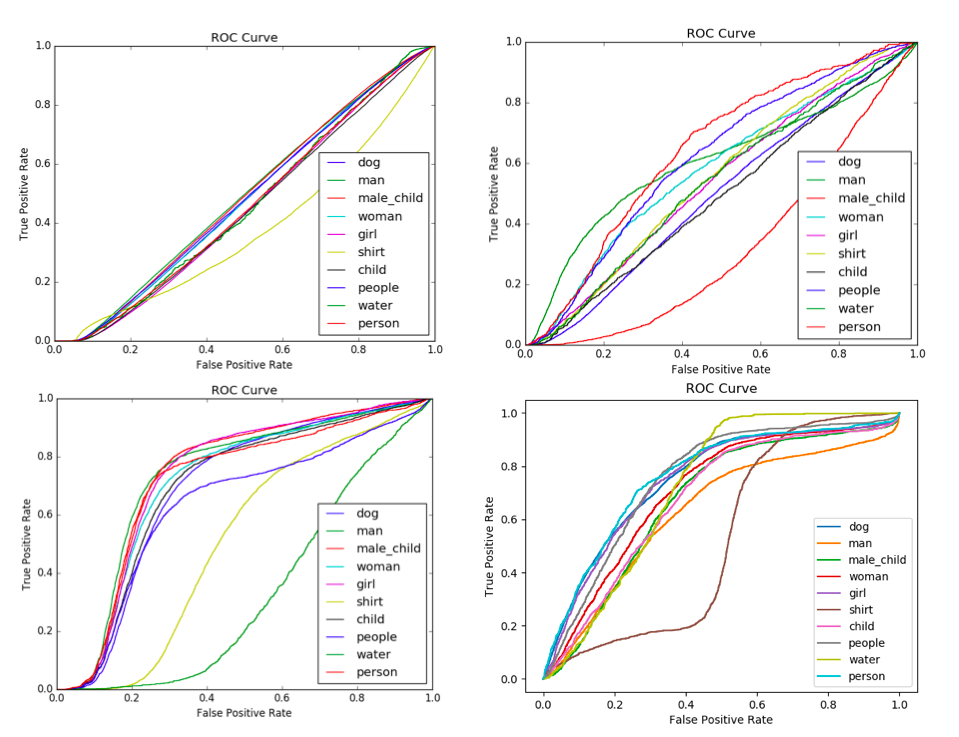
\includegraphics[width=0.8\textwidth]{fig_4.png}
    \caption{ROC for audio-level models. Bottom-left: The framewise GMM with MFCC; the pre-segmented GMM with MFCC; the pre-segmented HMM with MFCC; ES-KMeans with bottleneck features.}
    \label{fig:roc_audio}
\end{figure*}

\begin{figure*}[t]
    \centering
    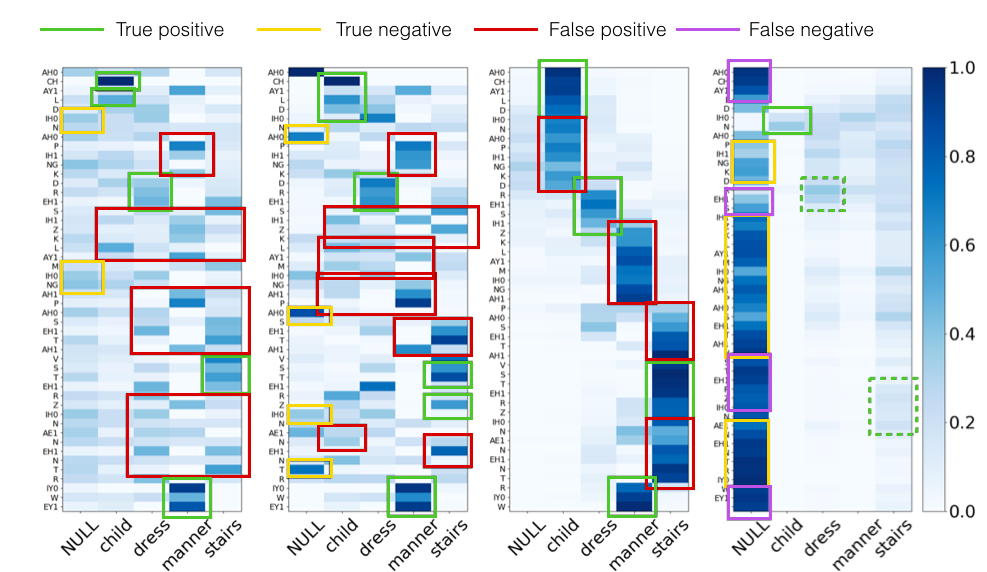
\includegraphics[width=0.9\textwidth]{fig_8.png}
    \caption{Attention/align probability matrices annotated with discovered word-like units of various phone-level models for the utterance ``A child in a pink dress is climbing pass the stairs of a entry way''. Leftmost: simplified mixture model; middle left: enriched mixture model; middle right: segmental model; rightmost: NMT}
    \label{fig:attention_plots}
\end{figure*}

\begin{figure*}[t]
    \centering
    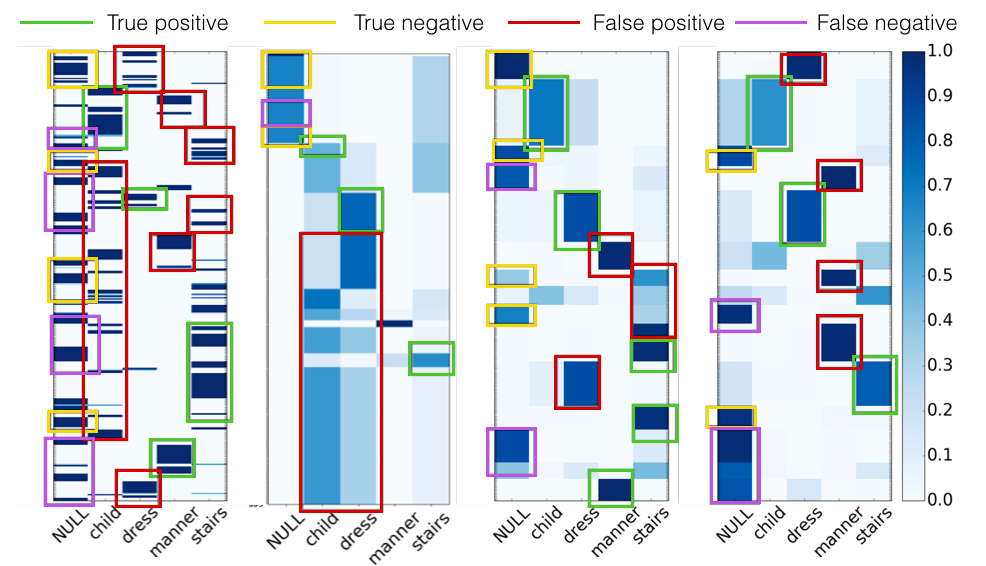
\includegraphics[width=0.9\textwidth]{fig_9.png}
    \caption{Align probability matrices annotated with discovered word-like units of various audio-level models for the utterance ``A child in a pink dress is climbing pass the stairs of a entry way''. Leftmost: enriched mixture model with BN feature; middle left: dynamic segmental KMeans; middle right: static segmental GMM; rightmost: static segmental HMM}
    \label{fig:audio_alignprob_plots}
\end{figure*}

The phone-level word discovery results are summarized in Table. (\ref{tab:phone_level_result}).
From the retrieval based scores, we see that segmental model is better at aligning phone to image concepts as it performs better in both recall and precision than the simplified model. The enriched model, however performs worse than the simplified model potentially because the image concepts do not appear in approximately the same order as the corresponding words in the utterances. 

The alignment probability/attention matrices for the four models are shown in Fig. (\ref{fig:attention_plots}). For the segmental model, the alignment probabilities are defined as the Viterbi probabilities normalized across concepts at a given time.  From the alignment probability, we notice that the segmental model has much sparser alignment probabilities and produces much more continuous pseudo-words that are closer the length of a real word, suggesting that contextual information between phones is crucial for discovering word-like units. However, the segmental model seems to be worse at distinguishing \texttt{NULL} from actual concepts, making many false positives, indicating that the \texttt{NULL} concept is statistically distinct from the rest of the concepts and should be modelled separately. Another cause of the false discovery stems from the limitation of a concept-independent jump transition probabilities: it appears that the segmental model prefers smaller jumps than larger ones, causing a exceedingly slow transition from one concept to another. This is evident from the example attention plot: almost every transition moves one step at a time. In particular, we can clearly see that the model stays at the concept ``child'' for eight extra phones until the align probability drops gradually. Another observation is that the accuracy of SMT is generally lower than the retrieval metrics as opposed to higher in the case of NMT primary because SMT is less biased towards concepts that appear more frequently while NMT tends to memorize the prior distribution of the concepts in the training data.

The ROC for the four models are shown in Fig. (\ref{fig:roc_phn}). All three SMT models are capable of detecting top concepts like ``man'', ``girl'', ``water'' and ``shirt'' with a nontrivial tradeoff between true positive rate and false positive rate. While both the simplified and segmental models have trouble discovering words for the extremely frequent concepts ``dog'', the enriched model is able to handle it more consistently. This difficulty is consistent with the previous hypothesis for why the accuracy score is lower than the retrieval metrics. Overall, the enriched model has the most consistent ROCs across different concepts. The ROC for the NMT has the highest variability across concepts. For concepts like ``dog'' and ``girl'', a higher attention weights seem to indicate the absence rather than the existence of the concept.    

%\begin{figure}
%    \centering
%    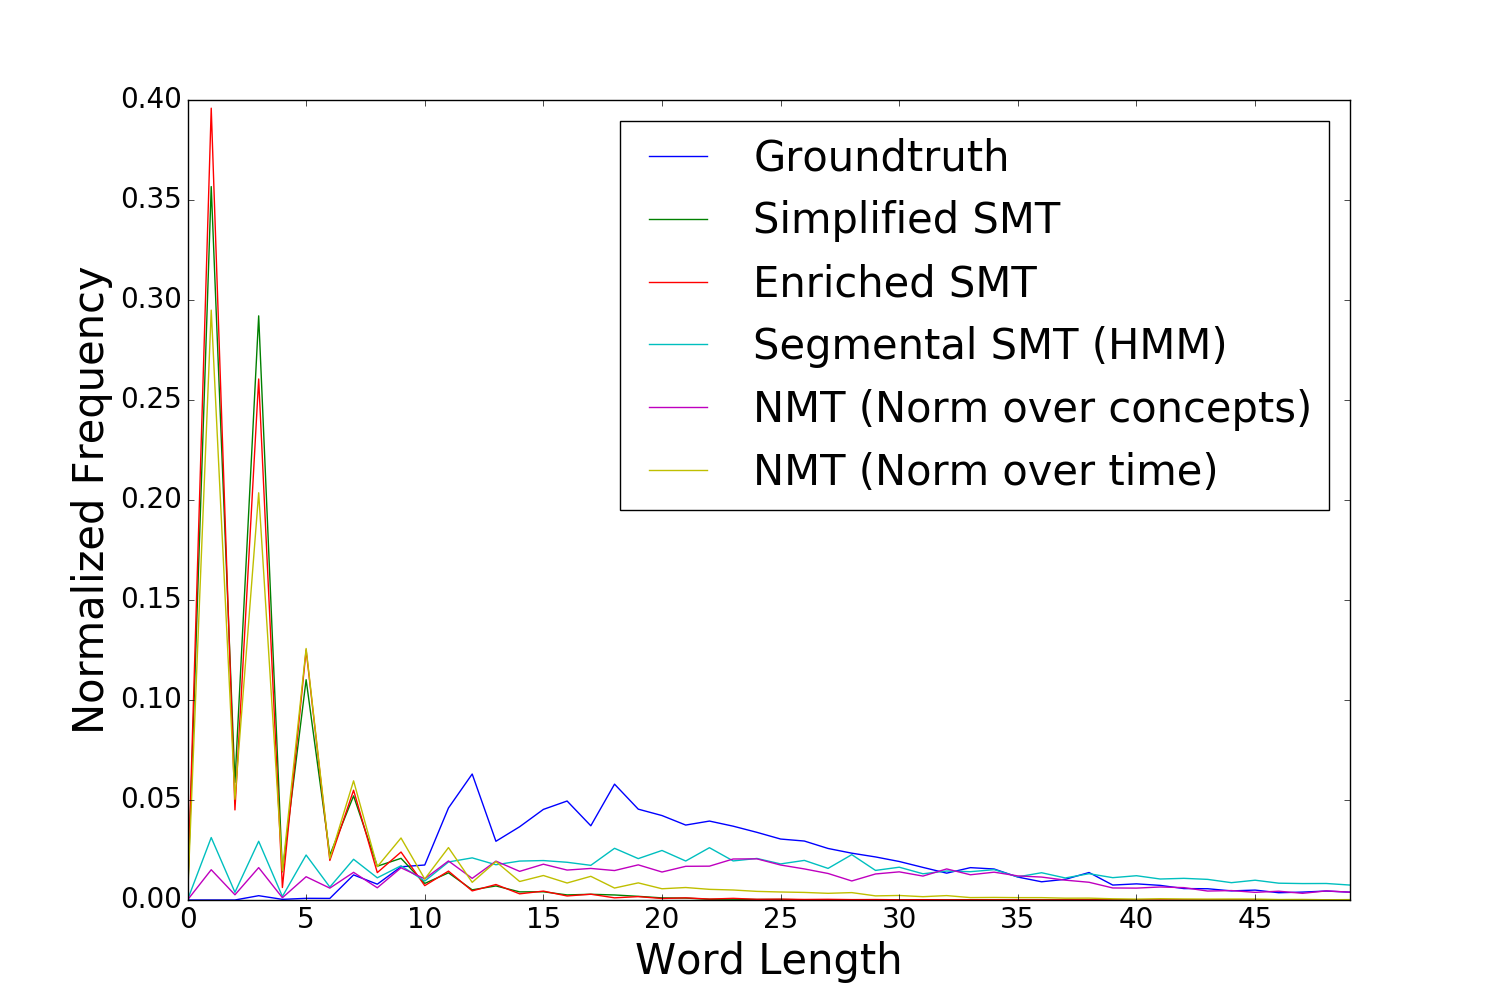
\includegraphics[width=0.5\textwidth]{fig_6.png}
%    \caption{Length Distribution for various phone-level models}
%    \label{fig:len_dist}
%\end{figure}
\begin{table}[t]
    \centering
    \begin{tabular}{|c|c|c|c|c|}
    \hline
    \multicolumn{2}{|c|}{}   &SylSeg &ES-KMeans & \begin{tabular}{@{}c@{}}
            Simplified\\
            Dynamic Segmental
        \end{tabular}\\
    \hline
    \multirow{2}{*}{Recall}  & MFCC & \multirow{2}{*}{83.5}  & 35.7   & 35.6  \\
            & BN    & & -  & 38.2  \\
    \hline
    \multirow{2}{*}{Precision} & MFCC &\multirow{2}{*}{33.9}   & 41.0  & 40.2  \\ 
    & BN    &  & - & 41.6  \\
    \hline
    \multirow{2}{*}{F1}  &  MFCC & \multirow{2}{*}{48.2} & 38.1  & 37.2  \\
        & BN    &      & -     & 39.9  \\
    \hline
    \end{tabular}
    \caption{audio-level word segmentation results}
    \label{tab:audio_seg_result}
\end{table}
\begin{table*}[t]
    \centering
    \begin{tabular}{|c|c|c|c|c|c|c|c|}
    \hline
\multicolumn{2}{|c|}{} & \begin{tabular}{@{}c@{}}
     Simplified \\
     Mixture
\end{tabular} & \begin{tabular}{@{}c@{}}
     Enriched\\
     Mixture
\end{tabular} &  \begin{tabular}{@{}c@{}}
          Static Segmental \\
          GMM
\end{tabular} & \begin{tabular}{@{}c@{}}
          Static Segmental \\
          HMM
\end{tabular} & \begin{tabular}{@{}c@{}}
     Simplified Dynamic \\
     Segmental
\end{tabular} & \begin{tabular}{@{}c@{}}NMA \\
(Normalized ov. Concept)\end{tabular}\\
\hline
\multirow{2}{*}{Accuracy} & MFCC & 32.2 & 27.1  & 36.6  & 31.2  &  28.0 & 19.3  \\
& BN    & 35.6  &  36.6 & $\mathbf{40.8}$  & 37.9  & 29.7 & 20.3 \\
\hline
\multirow{2}{*}{Recall} & MFCC  & 30.4  & 27.5  & 36.1  & 32.7  & 26.2  & 25.7 \\
                        & BN    & 36.5 & 36.4  & $\mathbf{44.1}$    & 39.7  & 37.4  & 27.0  \\
\hline
\multirow{2}{*}{Precision} & MFCC  & 29.8  & 26.9 & 34.7 & 30.6   & 23.9  & 12.2  \\
                           & BN    & 34.6 & 34.3 & $\mathbf{40.5}$ & 36.5   & 39.4  &  13.3 \\
\hline
\multirow{2}{*}{F1} & MFCC  & 30.1  & 27.2  & 35.4  & 31.6  & 25.0  & 23.1  \\
                    & BN    & 35.5 &  35.3  & $\mathbf{42.3}$  & 38.0  & 38.3  & 17.8  \\
\hline
\multirow{2}{*}{\begin{tabular}{@{}c@{}}
     Avg. Word Length\\
     (True Avg. = 61.2)
\end{tabular}} & MFCC & 3.14  & 3.26  & 39.9  & 40.8  & 140.1  & 36.9  \\
                                   & BN    & 6.32  & 6.31  & 42.2  & 39.9   & $\mathbf{71.8}$   & 16.0  \\
\hline
\end{tabular}
    \caption{Audio-level Word Discovery Results}
    \label{tab:audio_level_result}
\end{table*}
\subsubsection{Audio-level discovery}
The Tab. (\ref{tab:audio_level_result}) shows the audio-level word discovery results. Segmental models generally outperforms the simplified model approaches and produce words more realistic lengths. The static segmental models generally performs better than the dynamic model when using MFCC. The static segmental GMM performs best when using either MFCC or BN, suggesting that the dynamic segmentation may be unnecessary for our dataset since most words has one or two syllables. This is also consistent with the observation that the Markov assumption does not boost the performance of word discovery, suggesting that different syllables in the speech is weakly correlated. The Dynamic segmental model produces words of the most realistic lengths when using BN but tend to under-segment and create extremely long segment when using MFCC. The bottleneck feature performs significantly better than the MFCC in all models possibly by incorporating more contextual information. The overall result shows a dramatic drop in performance compared to the phone-level case, possibly because of the aliasing introduced by the resampled embedding approach, the speaker variability and other loss of information during the feature extraction process. Indeed, from Table. (\ref{tab:audio_seg_result}), features seem to subvert the segmentation process since the feature-free SylSeg model has a higher F1 scores than the feature-dependent ES-KMeans model and Multimodal ES-Kmeans model, while the similar phone-level mixture models are likely to improve the F-score given a pre-segmentation. 

The ROC curves for the audio-level word-discovery results are shown in Fig. (\ref{fig:roc_audio}). The frame-wise approach performs almost at chance level and does  not make any nontrivial discoveries. The problem is mitigated by the pre-segmented GMM and starts to have above-random performance detecting concepts like ``male-child'' and ``man''; the pre-segmented HMM further improves the discovery of common concepts by incorporating contextual information from the neighboring syllables, but miss many occurrences of concepts ``shirt'' and ``man''. The dynamic refinement of segmentation by ESKMeans also helps the detection of common concepts but interestingly, also having trouble discovering the concept ``shirt''.   

The align probability matrices for four audio-level models are shown in Fig. (\ref{fig:audio_alignprob_plots}). Different from phone-level plots, the plots are not generated by exponentiating the raw translation probabilities but a smoothed version with some temperature $T$:
\begin{align*}
    p'(i(t)|\mathbf x, \mathbf y) = \frac{\exp(\log p(i(t)|\mathbf x, \mathbf y)/T)}{\sum_i \exp(\log p(i'|\mathbf x, \mathbf y)/T)}.
\end{align*}
The smoothing does not alter the trend of the probabilities but make it more visually informative. We found $T=1000$ to work well generally. Judged from the plots, the two static segmental models perform similarly in true discoveries and the HMM tend to discover more continuous words, but the HMM has more false positives and false negatives. Indeed, all except the static segmental HMM model clusters the first few frames of silence to \texttt{NULL} symbol. Overall, most models display a high level of false discoveries, possibly because statistical property of \texttt{NULL} symbol is different from other concepts in that it is more dependent on the type of concepts present in an image. Further, the dramatic drop in F1 score indicates that the audio-level models are having troubles extracting the phonetic information from audio that is necessary to reduce the problem to the phone-level discovery. 

\subsubsection{Phone-to-concept retrieval}
The result for phone-to-concept retrieval compared with the speech-to-image and text-to-image systems are shown in Table. (\ref{tab:retrieval_results}). The performance of the simplified SMA retriever is just in between its speech-to-image and the text-to-image counterparts while the segmental SMA retriever performs much better than other models in all recall scores, partly due to the use of groundtruth hard labels for both the speech and image. It demonstrates that detecting the entities is the key for the image retrieval task on our dataset. Nevertheless, many of the errors made by our systems come from either unknown image concepts or image with very similar top concepts, so there is a substantial room for improvement on the concept level,  especially in making use of the contextual information between concepts in retrieval. For example, the concept ``shirt'' and ``hand'' are more likely when a person is present. Indeed, the SMA-based retriever does not perform well in our preliminary experiments for the more challenging task of captioning primarily due to the lack of modeling between the relation between concepts.  

\begin{table}[t]
    \centering
    \begin{tabular}{|c|c|c|c|}
    \hline
        & Recall@1  & Recall@5   & Recall@10  \\
    \hline
        Simplified SMT & 9.42\% & 21.1\% & 29.1\% \\
        Segmental SMT & 46.7\% & 65.2\%  & 72.2\%  \\
        Harwath\&Glass\cite{Harwath15} & - & - & 17.9\%\\
        Karpathy\cite{Karpathy15} & 10.3\% & 31.4\% & 42.5\%\\
    \hline
    \end{tabular}
    \caption{Comparison of query-by-example image search with spoken/phone sequence result}
    \label{tab:retrieval_results}
\end{table}
% An example of a floating figure using the graphicx package.
% Note that \label must occur AFTER (or within) \caption.
% For figures, \caption should occur after the \includegraphics.
% Note that IEEEtran v1.7 and later has special internal code that
% is designed to preserve the operation of \label within \caption
% even when the captionsoff option is in effect. However, because
% of issues like this, it may be the safest practice to put all your
% \label just after \caption rather than within \caption{}.
%
% Reminder: the "draftcls" or "draftclsnofoot", not "draft", class
% option should be used if it is desired that the figures are to be
% displayed while in draft mode.
%
%\begin{figure}[!t]
%\centering
%\includegraphics[width=2.5in]{myfigure}
% where an .eps filename suffix will be assumed under latex, 
% and a .pdf suffix will be assumed for pdflatex; or what has been declared
% via \DeclareGraphicsExtensions.
%\caption{Simulation results for the network.}
%\label{fig_sim}
%\end{figure}

% Note that the IEEE typically puts floats only at the top, even when this
% results in a large percentage of a column being occupied by floats.


% An example of a double column floating figure using two subfigures.
% (The subfig.sty package must be loaded for this to work.)
% The subfigure \label commands are set within each subfloat command,
% and the \label for the overall figure must come after \caption.
% \hfil is used as a separator to get equal spacing.
% Watch out that the combined width of all the subfigures on a 
% line do not exceed the text width or a line break will occur.
%
%\begin{figure*}[!t]
%\centering
%\subfloat[Case I]{\includegraphics[width=2.5in]{box}%
%\label{fig_first_case}}
%\hfil
%\subfloat[Case II]{\includegraphics[width=2.5in]{box}%
%\label{fig_second_case}}
%\caption{Simulation results for the network.}
%\label{fig_sim}
%\end{figure*}
%
% Note that often IEEE papers with subfigures do not employ subfigure
% captions (using the optional argument to \subfloat[]), but instead will
% reference/describe all of them (a), (b), etc., within the main caption.
% Be aware that for subfig.sty to generate the (a), (b), etc., subfigure
% labels, the optional argument to \subfloat must be present. If a
% subcaption is not desired, just leave its contents blank,
% e.g., \subfloat[].


% An example of a floating table. Note that, for IEEE style tables, the
% \caption command should come BEFORE the table and, given that table
% captions serve much like titles, are usually capitalized except for words
% such as a, an, and, as, at, but, by, for, in, nor, of, on, or, the, to
% and up, which are usually not capitalized unless they are the first or
% last word of the caption. Table text will default to \footnotesize as
% the IEEE normally uses this smaller font for tables.
% The \label must come after \caption as always.
%
%\begin{table}[!t]
%% increase table row spacing, adjust to taste
%\renewcommand{\arraystretch}{1.3}
% if using array.sty, it might be a good idea to tweak the value of
% \extrarowheight as needed to properly center the text within the cells
%\caption{An Example of a Table}
%\label{table_example}
%\centering
%% Some packages, such as MDW tools, offer better commands for making tables
%% than the plain LaTeX2e tabular which is used here.
%\begin{tabular}{|c||c|}
%\hline
%One & Two\\
%\hline
%Three & Four\\
%\hline
%\end{tabular}
%\end{table}


% Note that the IEEE does not put floats in the very first column
% - or typically anywhere on the first page for that matter. Also,
% in-text middle ("here") positioning is typically not used, but it
% is allowed and encouraged for Computer Society conferences (but
% not Computer Society journals). Most IEEE journals/conferences use
% top floats exclusively. 
% Note that, LaTeX2e, unlike IEEE journals/conferences, places
% footnotes above bottom floats. This can be corrected via the
% \fnbelowfloat command of the stfloats package.

\section{Conclusion}
This paper describes a unified framework for multimodal word discovery with spoken captions and image concepts. Four systems were tested with three different representations of the spoken caption: the groundtruth phonetic labels, MFCC and MBN. With the amount of data we have, the segmental SMT approach performs best in the phone-level while the enriched SMT performs best in the audio-level, according to our evaluation metrics. We applied our word discovery system to the task of image retrieval and show that the segmental SMT-based system achieves $72.2 \%$ recall@10 score in the phone-level. However, the drop in performance of all systems in the audio-level suggests a urgent need for better unsupervised phone-level and syllable-level representation for spoken language.  





% if have a single appendix:
%\appendix[Proof of the Zonklar Equations]
% or
%\appendix  % for no appendix heading
% do not use \section anymore after \appendix, only \section*
% is possibly needed

% use appendices with more than one appendix
% then use \section to start each appendix
% you must declare a \section before using any
% \subsection or using \label (\appendices by itself
% starts a section numbered zero.)
%


\appendices
\section{}


% use section* for acknowledgment
\section*{Acknowledgment}



% Can use something like this to put references on a page
% by themselves when using endfloat and the captionsoff option.
\ifCLASSOPTIONcaptionsoff
  \newpage
\fi



% trigger a \newpage just before the given reference
% number - used to balance the columns on the last page
% adjust value as needed - may need to be readjusted if
% the document is modified later
%\IEEEtriggeratref{8}
% The "triggered" command can be changed if desired:
%\IEEEtriggercmd{\enlargethispage{-5in}}

% references section

% can use a bibliography generated by BibTeX as a .bbl file
% BibTeX documentation can be easily obtained at:
% http://mirror.ctan.org/biblio/bibtex/contrib/doc/
% The IEEEtran BibTeX style support page is at:
% http://www.michaelshell.org/tex/ieeetran/bibtex/
%\bibliographystyle{IEEEtran}
% argument is your BibTeX string definitions and bibliography database(s)
\bibliographystyle{IEEEtran}
\bibliography{sp2019_refs}

% that's all folks
\end{document}